\chapter{QMCPACK design and feature documentation}
\label{chap:design_features}

This section contains information on the overall design of QMCPACK.  Also included are detailed explanations/derivations of major features and algorithms present in the code.


\section{QMCPACK Design}
TBD.



\newpage
\section{Feature: Optimized long-range breakup (Ewald)}

% Written by Ken Esler as part of the Common codebase used in wfconvert
% Originally titled ``Ewald Breakup for Long-Range Potentials in PIMC''
% PIMC-specific portions have been commented out

Consider a group of particles interacting with long-range central
potentials, $v^{\alpha \beta}(|r^{\alpha}_i - r^{\beta}_j|)$, where the Greek superscripts
represent the particle species (e.g., $\alpha=\text{electron}$,
$\beta=\text{proton}$), and Roman subscripts refer to particle number
within a species.  We can then write the total interaction energy for
the system as
\newcommand{\vr}{\mathbf{r}}
\newcommand{\vR}{\mathbf{R}}
\newcommand{\vk}{\mathbf{k}}
\newcommand{\vq}{\mathbf{q}}
\begin{equation}
V = \sum_\alpha \left\{\sum_{i<j} v^{\alpha\alpha}(|\vr^\alpha_i - \vr^\alpha_j|) +
\sum_{\beta<\alpha} 
\sum_{i,j} v^{\alpha \beta}(|\vr^{\alpha}_i - \vr^{\beta}_j|) \right\}
\label{eq:Vperiodic}\:.
\end{equation}
\newcommand{\va}{\mathbf{a}}
\newcommand{\vb}{\mathbf{b}}
\newcommand{\vL}{\mathbf{L}}

\subsection{The long-range problem}
Consider such a system in periodic boundary conditions in a cell
defined by primitive lattice vectors $\va_1$, $\va_2$, and $\va_3$.
Let $\vL \equiv n_1 \va_1 + n_2 \va_2 + n_3\va_3$ be a direct lattice
vector.  Then the interaction energy per cell for the periodic system
is given by
\begin{equation}
\begin{split}
V = & \sum_\vL \sum_\alpha \left\{ 
\overbrace{\sum_{i<j} v^{\alpha\alpha}(|\vr^\alpha_i - \vr^\alpha_j + \vL|)}^{\text{homologous}} +
\overbrace{\sum_{\beta<\alpha} 
\sum_{i,j} v^{\alpha \beta}(|\vr^{\alpha}_i - \vr^{\beta}_j+\vL|)}^{\text{heterologous}}
\right\}  \\
& + \underbrace{\sum_{\vL \neq \mathbf{0}} \sum_\alpha N^\alpha v^{\alpha \alpha} (|\vL|)}_\text{Madelung}\:.
\end{split}
\label{eq:direct}\:,
\end{equation}
where $N^\alpha$ is the number particles of species $\alpha$.
If the potentials $v^{\alpha\beta}(r)$ are indeed long-range, the
summation over direct lattice vectors will not converge in this naive
form.  A solution to the problem was posited by Ewald.  We break the
central potentials into two pieces---a short-range and a long-range
part defined by
\begin{equation}
v^{\alpha \beta}(r) = v_s^{\alpha\beta}(r) + v_l^{\alpha \beta}(r)\:.
\end{equation}
We will perform the summation over images for the short-range part in
real space, while performing the sum for the long-range part in
reciprocal space.  For simplicity, we choose $v^{\alpha \beta}_s(r)$
so that it is identically zero at the half-the-box length.  This
eliminates the need to sum over images in real space.


\subsection{Reciprocal-space sums}
\subsubsection{Heterologous terms}
We begin with Equation~\ref{eq:direct}, starting with the heterologous terms (i.e., the terms involving particles of different species).  The
short-range terms are trivial, so we neglect them here.
\begin{equation}
\text{heterologous} = \frac{1}{2} \sum_{\alpha \neq \beta} \sum_{i,j} \sum_\vL
v^{\alpha\beta}_l(\vr_i^\alpha - \vr_j^\beta + \vL)\:.
\end{equation}
We insert the resolution of unity in real space twice:
\begin{eqnarray}
\text{heterologous} & = & \frac{1}{2}\sum_{\alpha \neq \beta} \int_\text{cell} d\vr \, d\vr' \, \sum_{i,j}
\delta(\vr_i^\alpha - \vr) \delta(\vr_j^\beta-\vr') \sum_\vL
v^{\alpha\beta}_l(|\vr - \vr' + \vL|)\:, \\
& = & \frac{1}{2\Omega^2}\sum_{\alpha \neq \beta} \int_\text{cell} d\vr \, d\vr' \, \sum_{\vk, \vk', i, j} e^{i\vk\cdot(\vr_i^\alpha
  - \vr)} e^{i\vk'\cdot(\vr_j^\beta - \vr')} \sum_\vL
v^{\alpha\beta}_l(|\vr - \vr' + \vL|) \nonumber\:, \\
& = & \frac{1}{2\Omega^2} \sum_{\alpha \neq \beta} \int_\text{cell} d\vr \, d\vr'\,
\sum_{\vk, \vk', \vk'', i, j} e^{i\vk\cdot(\vr_i^\alpha - \vr)}
e^{i\vk'\cdot(\vr_j^\beta-\vr')} e^{i\vk''\cdot(\vr -\vr')}
v^{\alpha\beta}_{\vk''}\nonumber\:.
\end{eqnarray}
Here, the $\vk$ summations are over reciprocal lattice vectors given
by $\vk = m_1 \vb_1 + m_2\vb_2 + m_3\vb_3$, where
\begin{eqnarray}
\vb_1 & = & 2\pi \frac{\va_2 \times \va_3}{\va_1 \cdot (\va_2 \times
  \va_3)} \nonumber\:, \\
\vb_2 & = & 2\pi \frac{\va_3 \times \va_1}{\va_1 \cdot (\va_2 \times
  \va_3)}\:, \\
\vb_3 & = & 2\pi \frac{\va_1 \times \va_2}{\va_1 \cdot (\va_2 \times
  \va_3)} \nonumber\:.
\end{eqnarray}
We note that $\vk \cdot \vL = 2\pi(n_1 m_1 + n_2 m_2 + n_3 m_3)$. 
\begin{eqnarray}
v_{k''}^{\alpha \beta} & = & 
\frac{1}{\Omega} \int_{\text{cell}} d\vr'' \sum_\vL
e^{-i\vk''\cdot(|\vr''+\vL|)} v^{\alpha\beta}(|\vr''+\vL|)\:, \\
& = & \frac{1}{\Omega} \int_\text{all space} d\tilde{\vr} \, 
    e^{-i\vk'' \cdot \tilde{\vr}} v^{\alpha\beta}(\tilde{r})\:, \label{eq:vk}
\end{eqnarray}
where $\Omega$ is the volume of the cell. Here we have used the fact
that summing over all cells of the integral over the cell is
equivalent to integrating over all space.
\begin{equation}
\text{hetero} = \frac{1}{2\Omega^2} \sum_{\alpha \neq \beta}
\int_\text{cell} d\vr \, d\vr' \, \sum_{\vk, \vk', \vk'', i, j}
e^{i(\vk \cdot \vr_i^\alpha + \vk' \cdot\vr_j^\beta)} e^{i(\vk''-\vk)\cdot \vr}
e^{-i(\vk'' + \vk')\cdot \vr'} v^{\alpha \beta}_{\vk''}\:.
\end{equation}
We have
\begin{equation}
\frac{1}{\Omega} \int d\vr \  e^{i(\vk -\vk')\cdot \vr} =
\delta_{\vk,\vk'}\:.
\end{equation}
Then, performing the integrations we have
\begin{eqnarray}
\text{hetero} = \frac{1}{2} \sum_{\alpha \neq \beta}
\sum_{\vk, \vk', \vk'', i, j}
e^{i(\vk \cdot \vr_i^\alpha + \vk' \cdot\vr_j^\beta)} \delta_{\vk,\vk''}
\delta_{-\vk', \vk''} v^{\alpha \beta}_{\vk''}\:.
\end{eqnarray}
We now separate the summations, yielding
\begin{equation}
\text{hetero} = \frac{1}{2} \sum_{\alpha \neq \beta} \sum_{\vk, \vk'}
\underbrace{\left[\sum_i e^{i\vk  \cdot \vr_i^\alpha} \rule{0cm}{0.705cm}
    \right]}_{\rho_\vk^\alpha}
\underbrace{\left[\sum_j e^{i\vk' \cdot \vr_j^\beta} \right]}_{\rho_{\vk'}^\beta}
 \delta_{\vk,\vk''} \delta_{-\vk', \vk''} v^{\alpha
  \beta}_{\vk''}\:.
\end{equation}
Summing over $\vk$ and $\vk'$, we have
\begin{equation}
\text{hetero} = \frac{1}{2} \sum_{\alpha \neq \beta} \sum_{\vk''}
\rho_{\vk''}^\alpha \, \rho_{-\vk''}^\beta v_{k''}^{\alpha \beta}\:.
\end{equation}
We can simplify the calculation a bit further by rearranging the
sums over species:
\begin{eqnarray}
\text{hetero} & = & \frac{1}{2} \sum_{\alpha > \beta} \sum_{\vk}
\left(\rho^\alpha_\vk \rho^\beta_{-\vk} + \rho^\alpha_{-\vk}
\rho^\beta_\vk\right) v_{k}^{\alpha\beta}\:, \\
& = & \sum_{\alpha > \beta} \sum_\vk \mathcal{R}e\left(\rho_\vk^\alpha
\rho_{-\vk}^\beta\right)v_k^{\alpha\beta} .
\end{eqnarray}
\subsubsection{Homologous Terms}
We now consider the terms involving particles of the same species
interacting with each other.  The algebra is very similar to the
preceding, with the slight difficulty of avoiding the self-interaction term.
\begin{eqnarray}
\text{homologous} & = & \sum_\alpha \sum_L \sum_{i<j} v_l^{\alpha
  \alpha}(|\vr_i^\alpha - \vr_j^\alpha + \vL|)\:, \\
 & = & \frac{1}{2} \sum_\alpha \sum_L \sum_{i\neq j} v_l^{\alpha
  \alpha}(|\vr_i^\alpha - \vr_j^\alpha + \vL|)\:. 
\end{eqnarray}
\begin{eqnarray}
\text{homologous} & = & \frac{1}{2} \sum_\alpha \sum_L 
\left[
-N^\alpha v_l^{\alpha \alpha}(|\vL|)  + \sum_{i,j} v^{\alpha \alpha}_l(|\vr_i^\alpha - \vr_j^\alpha + \vL|)
  \right]\:, \\
& = & \frac{1}{2} \sum_\alpha \sum_\vk \left(|\rho_k^\alpha|^2 - N
\right) v_k^{\alpha \alpha}\:.
\end{eqnarray}
\subsubsection{Madelung terms}
Let us now consider the Madelung term for a single particle of species
$\alpha$.  This term corresponds to the interaction of a particle with
all of its periodic images.  
\begin{eqnarray}
v_M^{\alpha} & = & \frac{1}{2} \sum_{\vL \neq \mathbf{0}} v^{\alpha
  \alpha}(|\vL|)\:, \\
& = & \frac{1}{2} \left[ -v_l^{\alpha \alpha}(0) + \sum_\vL v^{\alpha
  \alpha}(|\vL|) \right]\:, \\
& = & \frac{1}{2} \left[ -v_l^{\alpha \alpha}(0) + \sum_\vk v^{\alpha
  \alpha}_\vk \right]\:.  
\end{eqnarray}
\subsubsection{$\vk=\mathbf{0}$ terms}
Thus far, we have neglected what happens at the special point $\vk =
\mathbf{0}$.  For many long-range potentials, such as the Coulomb
potential, $v_k^{\alpha \alpha}$ diverges for $k=0$.  However, we
recognize that for a charge-neutral system, the divergent part of the
terms cancel each other.  If all the potential in the system were
precisely Coulomb, the $\vk=\mathbf{0}$ terms would cancel precisely,
yielding zero.  For systems involving PPs, however, it
may be that the resulting term is finite, but nonzero.  Consider
the terms from $\vk=\mathbf{0}$:
\begin{eqnarray}
V_{k=0} & = & \sum_{\alpha>\beta} N^\alpha N^\beta v^{\alpha \beta}_{k=0}
+ \frac{1}{2} \sum_\alpha \left(N^{\alpha}\right)^2 v^{\alpha\alpha}_{k=0}\:, \\
& = & \frac{1}{2} \sum_{\alpha,\beta} N^\alpha N^\beta v^{\alpha
  \beta}_{k=0}\:.
\label{eq:kzero}
\end{eqnarray}
Next, we must compute $v^{\alpha \beta}_{k=0}$.  
\begin{equation}
v^{\alpha \beta}_{k=0} = \frac{4 \pi}{\Omega} \int_0^\infty dr\ r^2
v_l^{\alpha \beta}(r)\:.
\end{equation}
We recognize that this integral will not converge because of the
large-$r$ behavior.  However, we recognize that when we do the sum in
Equation~\ref{eq:kzero}, the large-$r$ parts of the integrals will cancel
precisely.  Therefore, we define
\begin{equation}
\tilde{v}^{\alpha \beta}_{k=0} = \frac{4 \pi}{\Omega} 
\int_0^{r_\text{end}} dr\ r^2 v_l^{\alpha \beta}(r)\:,
\end{equation}
where $r_{\text{end}}$ is some cutoff value after which the potential
tails precisely cancel.
\subsubsection{Neutralizing background terms}
For systems with a net charge, such as the one-component plasma
(jellium), we add a uniform background charge, which makes the system
neutral.  When we do this, we must add a term that comes from the
interaction of the particle with the neutral background.  It is a
constant term, independent of the particle positions.  In general, we
have a compensating background for each species, which largely cancels
out for neutral systems.
\begin{equation}
V_\text{background} = -\frac{1}{2} \sum_\alpha \left(N^\alpha\right)^2 
v^{\alpha \alpha}_{s\mathbf{0}}
-\sum_{\alpha > \beta} N_\alpha N_\beta
v^{\alpha\beta}_{s\mathbf{0}}\:,
\end{equation}
where $v^{\alpha \beta}_{s\mathbf{0}}$ is given by
\begin{eqnarray}
v^{\alpha \beta}_{s\mathbf{0}} & = & \frac{1}{\Omega} \int_0^{r_c} d^3 r\ 
v^{\alpha \beta}_s(r)\:, \\
& = & \frac{4 \pi}{\Omega} \int_0^{r_c} r^2 v_s(r) \ dr \nonumber\:.
\end{eqnarray}


\subsection{Combining terms}
Here, we sum all of the terms we computed in the previous sections:
\begin{eqnarray}
V & = & \sum_{\alpha > \beta} \left[\sum_{i,j} v_s(|\vr_i^\alpha
  -\vr_j^\beta|) + \sum_\vk \mathcal{R}e\left(\rho_\vk^\alpha
  \rho_{-\vk}^\beta\right)v^{\alpha\beta}_k  -N^\alpha N^\beta
  v^{\alpha \beta}_{s\mathbf{0}}  \right] \nonumber\:, \\
& + & \sum_\alpha \left[ N^\alpha v_M^\alpha + \sum_{i>j} v_s(|\vr_i^\alpha -
  \vr_j^\alpha|) + \frac{1}{2} \sum_\vk \left( |\rho_\vk^\alpha|^2 -
  N\right) v^{\alpha\alpha}_\vk -\frac{1}{2}\left(N_\alpha\right)^2 v_{s\mathbf{0}}^{\alpha\alpha}\right] \nonumber\:, \\
& = & \sum_{\alpha > \beta} \left[\sum_{i,j} v_s(|\vr_i^\alpha
  -\vr_j^\beta|) + \sum_\vk \mathcal{R}e\left(\rho_\vk^\alpha
  \rho_{-\vk}^\beta\right) v^{\alpha \beta}_k   -N^\alpha N^\beta
  v^{\alpha \beta}_{s\mathbf{0}}  +\tilde{V}_{k=0} \right]\:, \\
& + & \sum_\alpha \left[ -\frac{N^\alpha v_l^{\alpha \alpha}(0)}{2}  + \sum_{i>j} v_s(|\vr_i^\alpha -
  \vr_j^\alpha|) + \frac{1}{2} \sum_\vk |\rho_\vk^\alpha|^2 v^{\alpha\alpha}_\vk - \frac{1}{2}\left(N_\alpha\right)^2
  v_{s\mathbf{0}}^{\alpha\alpha} +\tilde{V}_{k=0}\right]  \nonumber\:.
\end{eqnarray}

\subsection {Computing the reciprocal potential}
Now we return to Equation~\ref{eq:vk}.  Without loss of generality, we define
for convenience $\vk = k\hat{\mathbf{z}}$.
\begin{equation}
v^{\alpha \beta}_k = \frac{2\pi}{\Omega} \int_0^\infty dr \int_{-1}^1
  d\cos(\theta) \ r^2 e^{-i k r \cos(\theta)} v_l^{\alpha \beta}(r)\:.
\end{equation}
We do the angular integral first.  By inversion symmetry, the
imaginary part of the integral vanishes, yielding
\begin{equation}
v^{\alpha \beta}_k = \frac{4\pi}{\Omega k}\int _0^\infty dr\ r \sin(kr)
v^{\alpha \beta}_l(r)\:.
\label{eq:vkint}
\end{equation}
\subsection{The Coulomb potential}
For the case of the Coulomb potential, the preceding integral is not
formally convergent if we do the integral naively. We may remedy the
situation by including a convergence factor, $e^{-k_0 r}$.  For a
potential of the form $v^{\text{coul}}(r) = q_1 q_2/r$, this yields
\begin{eqnarray}
v^{\text{screened coul}}_k & = & \frac{4\pi q_1 q_2}{\Omega k} \int_0^\infty dr\ \sin(kr)
e^{-k_0r}\:, \\ 
& = & \frac{4\pi q_1 q_2}{\Omega (k^2 + k_0^2)}\:.
\end{eqnarray}
Allowing the convergence factor to tend to zero, we have
\begin{equation}
v_k^\text{coul} = \frac{4 \pi q_1 q_2}{\Omega k^2}\:.
\end{equation}

For more generalized potentials with a Coulomb tail, we cannot
evaluate Equation~\ref{eq:vkint} numerically but must handle the coulomb part
analytically.  In this case, we have
\begin{equation}
v_k^{\alpha \beta} = \frac{4\pi}{\Omega} 
\left\{ \frac{q_1 q_2}{k^2} + \int_0^\infty dr \ r \sin(kr) \left[ v_l^{\alpha \beta}(r) -
  \frac{q_1 q_2}{r} \right] \right\}\:.
\end{equation}

\subsection{Efficient calculation methods}
\subsubsection{Fast computation of $\rho_\vk$}
We wish to quickly calculate the quantity
\begin{equation}
\rho_\vk^\alpha \equiv \sum_i e^{i\vk \cdot r_i^\alpha}\:.
\end{equation}
First, we write 
\begin{eqnarray}
\vk & = & m_1 \vb_1 + m_2 \vb_2 + m_3 \vb_3\:, \\
\vk \cdot \vr_i^\alpha & = &  m_1 \vb_1 \cdot \vr_i^\alpha + 
m_2 \vb_2 \cdot \vr_i^\alpha + m_3 \vb_3 \cdot \vr_i^\alpha\:, \\
e^{i\vk \cdot r_i^\alpha} & = & 
{\underbrace{\left[e^{i \vb_1 \cdot\vr_i^\alpha}\right]}_{C^{i\alpha}_1}}^{m_1}
{\underbrace{\left[e^{i \vb_2 \cdot\vr_i^\alpha}\right]}_{C^{i\alpha}_2}}^{m_2}
{\underbrace{\left[e^{i \vb_3 \cdot\vr_i^\alpha}\right]}_{C^{i\alpha}_3}}^{m_3}\:.
\end{eqnarray}
Now, we note that
\begin{equation}
[C^{i\alpha}_1]^{m_1} = C^{i\alpha}_1 [C^{i\alpha}]^{(m_1-1)}\:.
\end{equation}
This allows us to recursively build up an array of the $C^{i\alpha}$s
and then compute $\rho_\vk$ for all $\vk$-vectors by looping over all
k-vectors, requiring only two complex multiplies per particle per
$\vk$.
\begin{algorithm}
\caption{Algorithm to quickly calculate $\rho_\vk^\alpha$.}
\begin{algorithmic}
\STATE Create list of $\vk$-vectors and corresponding $(m_1, m_2,
m_3)$ indices.
\FORALL{$\alpha \in $ species}
  \STATE Zero out $\rho_\vk^\alpha$
  \FORALL{$i \in $ particles}
    \FOR{$j \in [1\cdots3]$}
      \STATE Compute $C^{i \alpha}_j \equiv e^{i \vb_j \cdot
        \vr^{\alpha}_i}$
       \FOR{$m \in [-m_{\text{max}}\dots m_{\text{max}}]$}
         \STATE Compute $[C^{i \alpha}_j]^m$ and store in array
       \ENDFOR
    \ENDFOR
     \FORALL{$(m_1, m_2, m_3) \in $ index list}
       \STATE Compute $e^{i \vk \cdot r^\alpha_i} =
         [C^{i\alpha}_1]^{m_1} [C^{i\alpha}_2]^{m_2}
         [C^{i\alpha}_3]^{m_3}$ from array
    \ENDFOR
  \ENDFOR
\ENDFOR
\end{algorithmic}
\end{algorithm}

\subsection{Gaussian charge screening breakup}
This original approach to the short- and long-range breakup adds an
opposite screening charge of Gaussian shape around each point charge.
It then removes the charge in the long-range part of the potential.
In this potential,
\begin{equation}
v_{\text{long}}(r) = \frac{q_1 q_2}{r} \text{erf}(\alpha r)\:,
\end{equation}
where $\alpha$ is an adjustable parameter used to control how
short ranged the potential should be.  If the box size is $L$, a
typical value for $\alpha$ might be $7/(Lq_1 q_2)$. We should note
that this form for the long-range potential should also work for any
general potential with a Coulomb tail (e.g., pseudo-Hamiltonian
potentials.  For this form of the long-range potential, we have in $k$-space
\begin{equation}
v_k = \frac{4\pi q_1 q_2 \exp\left[\frac{-k^2}{4\alpha^2}\right]}{\Omega k^2}\:.
\end{equation}

\subsection{Optimized breakup method}
In this section, we undertake the task of choosing a
long-range/short-range partitioning of the potential, which is optimal
in that it minimizes the error for given real and $k$-space cutoffs
$r_c$ and $k_c$.  Here, we slightly modify the method introduced by
Natoli and Ceperley\cite{Natoli1995}. We choose $r_c =
\frac{1}{2}\min\{L_i\}$ so that we require the nearest image in
real-space summation.  $k_c$ is then chosen to satisfy our
accuracy requirements.

Here we modify our notation slightly to accommodate details not previously required.  We restrict our discussion to the interaction of two
particle species (which may be the same), and drop our species
indices.  Thus, we are looking for short- and long-range potentials
defined by
\renewcommand{\vs}{v^s}
\newcommand{\vl}{v^\ell}
\begin{equation}
v(r) = \vs(r) + \vl(r)\:.
\end{equation}
Define $\vs_k$ and $\vl_k$ to be the respective Fourier transforms of
the previous equation.  The goal is to choose $v_s(r)$ such that its value and
first two derivatives vanish at $r_c$, while making $\vl(r)$ as smooth as
possible so that $k$-space components, $\vl_k$, are very small for
$k>k_c$.  Here, we describe how to do this in an optimal way.

Define the periodic potential, $V_p$, as 
\begin{equation}
V_p(\vr) = \sum_l v(|\vr + \mathbf{l}|),
\end{equation}
where $\vr$ is the displacement between the two particles and
$\mathbf{l}$ is a lattice vector.  Let us then define our
approximation to this potential, $V_a$, as
\begin{equation}
V_a(\vr) = \vs(r) + \sum_{|\vk| < k_c} \vl_k e^{i\mathbf \vk \cdot \vr}\:.
\end{equation}
Now, we seek to minimize the RMS error over the cell,
\begin{equation}
\chi^2 = \frac{1}{\Omega}\int_\Omega d^3 \mathbf{r} \ 
\left| V_p(\vr) - V_a(\vr)\right|^2\:. 
\end{equation}
We may write
\begin{equation}
V_p(\vr) = \sum_{\vk} v_k e^{i \vk \cdot \vr}\:,
\end{equation}
where 
\begin{equation}
v_k = \frac{1}{\Omega} \int d^3\vr \ e^{-i\vk\cdot\vr}v(r)\:.
\end{equation}
We now need a basis in which to represent the broken-up potential.  We
may choose to represent either $\vs(r)$ or $\vl(r)$ in a real-space
basis.  Natoli and Ceperley chose the former in their paper.  We choose
the latter for a number of reasons.  First, singular potentials are
difficult to represent in a linear basis unless the singularity is
explicitly included.  This requires a separate basis for each type of
singularity.  The short-range potential may have an arbitrary number
of features for $r<r_c$ and still be a valid potential.  By
construction, however, we desire that $\vl(r)$ be smooth in real-space
so that its Fourier transform falls off quickly with increasing $k$.
We therefore expect that, in general, $\vl(r)$ should be
well represented by fewer basis functions than $\vs(r)$.  Therefore,
we define
\begin{equation}
\vl(r) \equiv
\begin{cases}
 \sum_{n=0}^{J-1} t_n h_n(r) & \text{for } r \le r_c \\
 v(r) & \text{for } r > r_c.
\end{cases}\:,
\end{equation}
where the $h_n(r)$ are a set of $J$ basis functions.  We require that
the two cases agree on the value and first two derivatives at $r_c$.
We may then define
\begin{equation}
c_{nk} \equiv \frac{1}{\Omega} \int_0^{r_c} d^3 \vr \ e^{-i\vk\cdot\vr} h_n(r)\:.
\end{equation}
Similarly, we define
\begin{equation}
x_k \equiv -\frac{1}{\Omega} \int_{r_c}^\infty d^3\vr \ e^{-i\vk\cdot\vr} v(r)\:.
\end{equation}
Therefore,
\begin{equation}
\vl_k = -x_k + \sum_{n=0}^{J-1} t_n c_{nk}\:. 
\end{equation}
Because $\vs(r)$ goes identically to zero at the box edge, inside the
cell we may write
\begin{equation}
\vs(\vr) = \sum_\vk \vs_k e^{i\vk \cdot \vr}\:.
\end{equation}
We then write
\begin{equation}
\chi^2 = \frac{1}{\Omega} \int_\Omega d^3 \vr \ 
\left| \sum_\vk e^{i\vk \cdot \vr} \left(v_k - \vs_k \right)
-\sum_{|\vk| \le k_c} \vl_k \right|^2\:.
\end{equation}
We see that if we define
\begin{equation}
\vs(r) \equiv v(r) - \vl(r)\:.
\end{equation}
Then
\begin{equation}
\vl_k + \vs_k = v_k\:,
\end{equation}
which then cancels out all terms for $|\vk| < k_c$.  Then we have
\begin{eqnarray}
\chi^2 & = & \frac{1}{\Omega} \int_\Omega d^3 \vr \ 
\left|\sum_{|\vk|>k_c} e^{i\vk\cdot\vr} 
\left(v_k -\vs_k \right)\right|^2\:, \\
& = & \frac{1}{\Omega} \int_\Omega d^3 \vr \ 
\left|\sum_{|\vk|>k_c} e^{i\vk\cdot\vr} \vl_k \right|^2\:, \\ 
& = & 
\frac{1}{\Omega} \int_\Omega d^3 \vr
\left|\sum_{|\vk|>k_c} e^{i\vk\cdot\vr}\left( -x_k + \sum_{n=0}^{J-1} t_n
c_{nk}\right) \right|^2\:.
\end{eqnarray}
We expand the summation,
\newcommand{\ns}{\negthickspace}
\begin{equation}
\chi^2 = \frac{1}{\Omega} \int_\Omega d^3 \vr \ns \ns \ns
\sum_{\{|\vk|,|\vk'|\}>k_c} \ns\ns\ns\ns\ns
 e^{i(\vk-\vk')\cdot \vr}
\left(x_k -\sum_{n=0}^{J-1} t_n c_{nk} \right)
\left(x_k -\sum_{m=0}^{J-1} t_{m} c_{mk'} \right)\:.
\end{equation}
We take the derivative w.r.t. $t_{m}$:
\begin{equation}
\frac{\partial (\chi^2)}{\partial t_{m}} =
\frac{2}{\Omega}\int_\Omega d^3 \vr \ns \ns \ns
\sum_{\{|\vk|,|\vk'|\}>k_c} \ns\ns\ns\ns\ns
 e^{i(\vk-\vk')\cdot \vr}
\left(x_k -\sum_{n=0}^{J-1} t_n c_{nk} \right) c_{mk'}\:.
\end{equation}
We integrate w.r.t. $\vr$, yielding a Kronecker $\delta$.
\begin{equation}
\frac{\partial (\chi^2)}{\partial t_{m}} =
2 \ns\ns\ns\ns\ns\ns\ns 
\sum_{\ \ \ \ \{|\vk|,|\vk'|\}>k_c} \ns\ns\ns\ns\ns\ns\ns \delta_{\vk, \vk'} 
\left(x_k -\sum_{n=0}^{J-1} t_n c_{nk} \right) c_{mk'}\:.
\end{equation}
Summing over $\vk'$ and equating the derivative to zero, we find the
minimum of our error function is given by
\begin{equation}
\sum_{n=0}^{J-1} \sum_{|\vk|>k_c} c_{mk}c_{nk} t_n = 
\sum_{|\vk|>k_c} x_k c_{mk}\:,
\end{equation}
which is equivalent in form to Equation~19 in \cite{Natoli1995}, where
we have $x_k$ instead of $V_k$.  Thus, we see that we can optimize
the short- or long-range potential simply by choosing to use
$V_k$ or $x_k$ in the preceding equation.  We now define
\begin{eqnarray}
A_{mn} & \equiv & \sum_{|\vk|>k_c} c_{mk} c_{nk}\:, \\
b_{m} & \equiv & \sum_{|\vk|>k_c} x_k c_{mk}\:.
\end{eqnarray}
Thus, it becomes clear that our minimization equations can be cast in
the canonical linear form
\newcommand{\bA}{\mathbf{A}}
\newcommand{\bU}{\mathbf{U}}
\newcommand{\bV}{\mathbf{V}}
\newcommand{\bb}{\mathbf{b}}
\newcommand{\bS}{\mathbf{S}}
\begin{equation}
\bA\mathbf{t} = \mathbf{b}\:.
\end{equation}

\subsubsection{Solution by SVD}
In practice, we note that the matrix $\bA$ frequently becomes singular
in practice.  For this reason, we use the singular value decomposition
to solve for $t_n$.  This factorization decomposes $A$ as
\begin{equation}
\bA = \bU \bS \bV^T\:,
\end{equation}
where $\bU^T\bU = \bV^T\bV = 1$ and $\bS$ is diagonal.  In this form, we have
\begin{equation}
\mathbf{t} = \sum_{i=0}^{J-1} \left( \frac{\bU_{(i)} \cdot
  \bb}{\bS_{ii}} \right) \bV_{(i)}\:,
\end{equation}
where the parenthesized subscripts refer to columns.  The advantage of
this form is that if $\bS_{ii}$ is zero or very near zero, the
contribution of the $i^{\text{th}}$ of $\bV$ may be neglected since
it represents a numerical instability and has little physical
meaning.  It represents the fact that the system cannot distinguish
between two linear combinations of the basis functions.  Using the SVD
in this manner is guaranteed to be stable.  This decomposition is
available in LAPACK in the DGESVD subroutine.

\subsubsection{Constraining Values}
Often, we wish to constrain the value of $t_n$ to have a fixed value
to enforce a boundary condition, for example.  To do this, we define
\begin{equation}
\bb' \equiv \vb - t_n \bA_{(n)}\:.
\end{equation}
We then define $\bA^*$ as $\bA$ with the $n^{\text{th}}$ row and column
removed and $\bb^*$ as $\vb'$ with the $n^{\text{th}}$ element removed.  Then
we solve the reduced equation $\bA^* \mathbf{t}^* = \bb^*$ and
finally insert $t_n$ back into the appropriate place in $\mathbf{t}^*$
to recover the complete, constrained vector $\mathbf{t}$.  This may be
trivially generalized to an arbitrary number of constraints.
\label{sec:contraints}

\subsubsection{The LPQHI basis}
The preceding discussion is general and independent of the basis used to
represent $\vl(r)$.  In this section, we introduce a convenient basis
of localized interpolant functions, similar to those used for
splines, which have a number of properties that are convenient for
our purposes.  

First, we divide the region from 0 to $r_c$ into $M-1$ subregions,
bounded above and below by points we term {\em knots}, defined by $r_j
\equiv j\Delta$, where $\Delta \equiv r_c/(M-1)$.  We then define
compact basis elements, $h_{j\alpha}$, which span the region
$[r_{j-1},r_{j+1}]$, except for $j=0$ and $j=M$.  For $j=0$, only the
region $[r_0,r_1]$, while for $j=M$, only $[r_{M-1}, r_M]$.  Thus, the
index $j$ identifies the knot the element is centered on, while $\alpha$
is an integer from 0 to 2 indicating one of three function shapes.
The dual index can be mapped to the preceding single index by the
relation $n = 3j + \alpha$.  The basis functions are then defined as
\begin{equation}
h_{j\alpha}(r) = 
\begin{cases}
\ \ \ \, \Delta^\alpha \, \, \sum_{n=0}^5 S_{\alpha n} 
\left( \frac{r-r_j}{\Delta}\right)^n,    & r_j < r \le r_{j+1} \\
(-\Delta)^\alpha \sum_{n=0}^5 S_{\alpha n} 
\left( \frac{r_j-r}{\Delta}\right)^n,    & r_{j-1} < r \le r_j \\
\quad\quad\quad\quad\quad 0, & \text{otherwise}\:,
\end{cases}
\end{equation}
where the matrix $S_{\alpha n}$ is given by
\begin{equation}
S = 
\left[\begin{matrix}
1 & 0 & 0 & -10 & 15 & -6 \\
0 & 1 & 0 & -6  &  8 & -3 \\
0 & 0 & \frac{1}{2} & -\frac{3}{2} & \frac{3}{2} & -\frac{1}{2}
\end{matrix}\right]\:.
\end{equation}
\begin{figure}
\begin{center}
  \ifdefined\HCode
  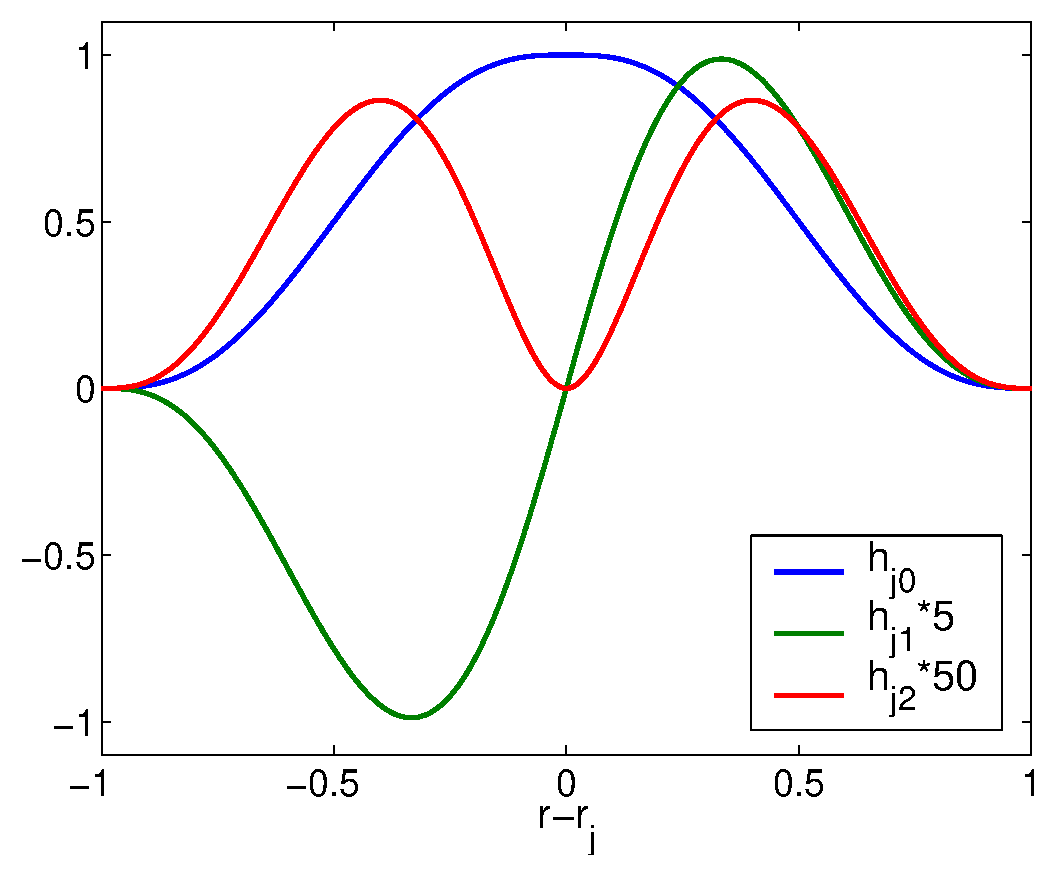
\includegraphics[width=3.5in]{./figures/LPQHI.dmn}
  \else
  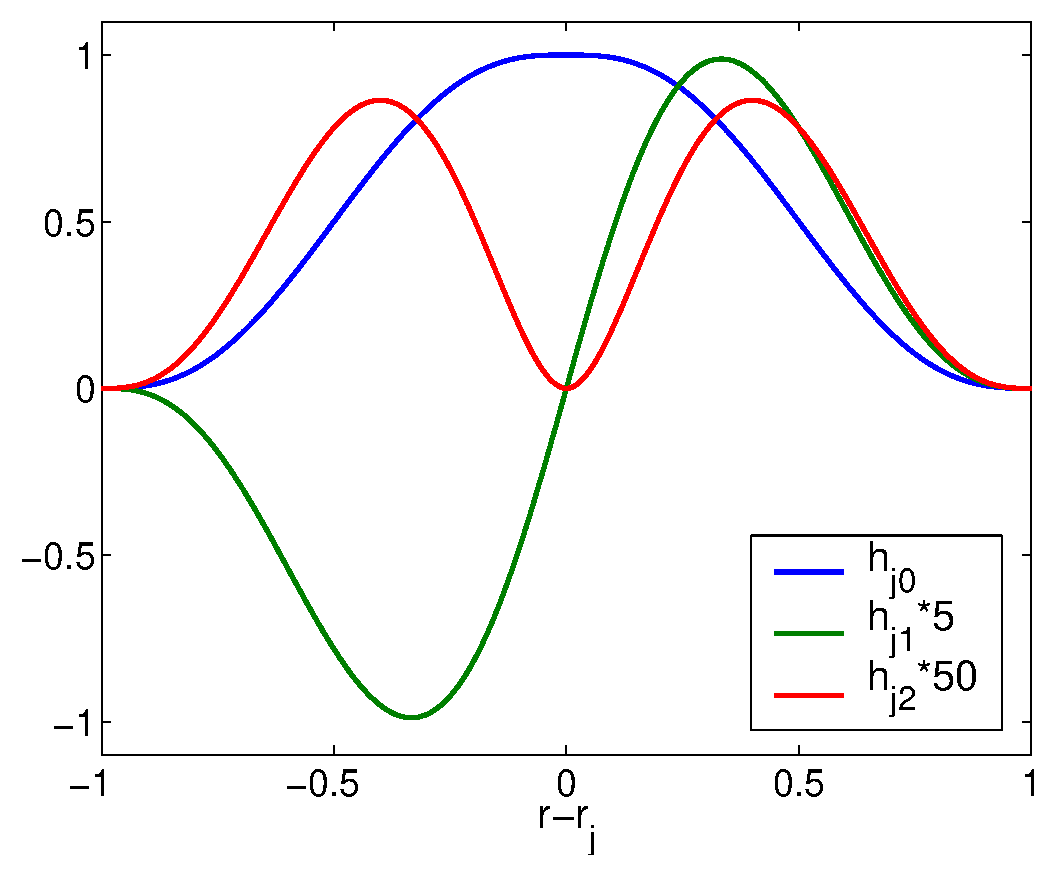
\includegraphics[width=3.5in]{./figures/LPQHI.pdf}
  \fi
\caption{Basis functions $h_{j0}$, $h_{j1}$, and $h_{j2}$ are shown.
We note that at the left and right extremes, the values and first two
derivatives of the functions are zero; while at the center, $h_{j0}$
has a value of 1, $h_{j1}$ has a first derivative of 1, and $h_{j2}$
has a second derivative of 1. }
\label{fig:LPQHI} 
\end{center}
\end{figure}
Figure~\ref{fig:LPQHI} shows plots of these function shapes.

The basis functions have the property that at the left and right
extremes (i.e., $r_{j-1}$ and $r_{j+1}$) their values and first two
derivatives are zero.  At the center, $r_j$, we have the properties
\begin{eqnarray}
h_{j0}(r_j)=1, & h'_{j0}(r_j)=0, & h''_{j0}(r_j)= 0\:, \\
h_{j1}(r_j)=0, & h'_{j1}(r_j)=1, & h''_{j1}(r_j)= 0\:, \\
h_{j2}(r_j)=0, & h'_{j2}(r_j)=0, & h''_{j2}(r_j)= 1\:. 
\end{eqnarray}
These properties allow the control of the value and first two derivatives
of the represented function at any knot value simply by setting the
coefficients of the basis functions centered around that knot.  Used
in combination with the method described in
Section~\ref{sec:contraints}, boundary conditions can easily be
enforced.  In our case, we wish require that
\begin{equation}
h_{M0} = v(r_c), \ \ h_{M1} = v'(r_c), \ \ \text{and} \ \  h_{M2} = v''(r_c)\:.
\end{equation}
This ensures that $\vs$ and its first two derivatives vanish at $r_c$.

\subsubsection*{Fourier coefficients}
We wish now to calculate the Fourier transforms of the basis
functions, defined as
\begin{equation}
c_{j\alpha k} \equiv \frac{1}{\Omega} \int_0^{r_c} d^3 \vr 
e^{-i \vk \cdot \vr} h_{j\alpha}(r)\:.
\end{equation}
We then may write,
\begin{equation}
c_{j\alpha k} = 
\begin{cases}
\Delta^\alpha \sum_{n=0}^5 S_{\alpha n} D^+_{0 k n}, & j = 0 \\
\Delta^\alpha \sum_{n=0}^5 S_{\alpha n} (-1)^{\alpha+n} D^-_{M k n}, &
j = M \\
\Delta^\alpha \sum_{n=0}^5 S_{\alpha n} 
\left[ D^+_{j k n} + (-1)^{\alpha+n}D^-_{j k n} \right] & \text{otherwise}\:,
\end{cases}
\end{equation}
where
\begin{equation}
D^{\pm}_{jkn} \equiv \frac{1}{\Omega} \int_{r_j}^{r_{j\pm1}} d^3\!\vr \ 
e^{-i\vk \cdot \vr} \left( \frac{r-r_j}{\Delta}\right)^n\:.
\end{equation}
We then further make the definition that
\renewcommand{\Im}{\text{Im}}
\begin{equation}
D^{\pm}_{jkn} = \pm \frac{4\pi}{k \Omega} 
\left[ \Delta \Im \left(E^{\pm}_{jk(n+1)}\right) + 
r_j \Im \left(E^{\pm}_{jkn}\right)\right]\:.
\end{equation}
It can then be shown that 
\begin{equation}
E^{\pm}_{jkn} =
\begin{cases}
-\frac{i}{k} e^{ikr_j} \left( e^{\pm i k \Delta} - 1 \right) &
\text{if } n=0, \\
-\frac{i}{k} 
\left[ \left(\pm1\right)^n e^{i k (r_j \pm \Delta)} - \frac{n}{\Delta}
E^\pm_{jk(n-1)}  \right] & \text{otherwise}\:.
\end{cases}
\end{equation}
Note that these equations correct typographical errors present in \cite{Natoli1995}.
\subsubsection{Enumerating $k$-points}
We note that the summations over $k$, which are ubiquitous in
this paper, require enumeration of the $k$-vectors.  In particular, we
should sum over all $|\vk| > k_c$.  In practice, we must limit our
summation to some finite cutoff value $k_c < |\vk| < k_{\text{max}}$,
where $k_{\text{max}}$ should be on the order of $3,000/L$, where $L$ is the
minimum box dimension.  Enumerating these vectors in a naive fashion
even for this finite cutoff would prove quite prohibitive, as it would 
require $\sim10^9$ vectors.

Our first optimization comes in realizing that all quantities in this
calculation require only $|\vk|$ and not $\vk$ itself.  Thus, we may
take advantage of the great degeneracy of $|\vk|$.  We create a list
of $(k,N)$ pairs, where $N$ is the number of vectors with magnitude $k$.
We make nested loops over
$n_1$, $n_2$, and $n_3$, yielding $\vk = n_1 \vb_1 + n_2 \vb_2 + n_3
\vb_3$. If $|\vk|$ is in the required range, we check to see whether there
is already an entry with that magnitude on our list and incremente the
corresponding $N$ if there is, or create a new entry if not.  Doing
so typically saves a factor of $\sim200$ in storage and computation.

This reduction is not sufficient for large $k_max$ since it
requires that we still look over $10^9$ entries.  To further reduce
costs, we may pick an intermediate cutoff, $k_{\text{cont}}$, above which
we will approximate the degeneracy assuming a continuum of
$k$-points.  We stop our exact enumeration at $k_{\text{cont}}$ and
then add $\sim1,000$ points, $k_i$, uniformly spaced between $k_{\text{cont}}$
and $k_{\text{max}}$. We then approximate the degeneracy by
\begin{equation}
N_i = \frac{4 \pi}{3} \frac{\left( k_b^3 -k_a^3\right)}{(2\pi)^3/\Omega}\:,
\end{equation}
where $k_b = (k_i + k_{i+1})/2$ and $k_a = (k_i + k_{i-1})$.  In doing
so, we typically reduce our total number of k-points to sum more than $\sim2,500$ from the $10^9$ we had to start.

\subsubsection{Calculating $x_k$'s}
\subsubsection*{The Coulomb potential}
For $v(r) = \frac{1}{r}$, $x_k$ is given by
\begin{equation}
x_k^{\text{coulomb}} = -\frac{4 \pi}{\Omega k^2} \cos(k r_c)\:.
\end{equation}

\subsection*{The $1/r^2$ potential}
For $v(r) = \frac{1}{r^2}$, $x_k$ is given by
\begin{equation}
x_k^{1/r^2} = \frac{4 \pi}{\omega k} 
\left[ \text{Si}(k r_c) -\frac{\pi}{2}\right],
\end{equation}
where the {\em sin integral}\:, $\text{Si}(z)$, is given by
\begin{equation}
\text{Si}(z) \equiv \int_0^z \frac{\sin \ t}{t} dt\:.
\end{equation}

\subsection*{The $1/r^3$ potential}
For $v(r) = \frac{1}{r^3}$, $x_k$ is given by
\begin{equation}
x_k^{1/r^3} = \frac{4\pi}{\Omega k} 
\left[k\text{Ci}(k r_c) - \frac{\sin(k r_c)}{r_c} \right]\:,
\end{equation}
where the {\em cosine integral}, $\text{Ci}(z)$, is given by
\begin{equation}
\text{Ci}(z) \equiv -\int_z^\infty \frac{\cos t}{t} dt\:.
\end{equation}

\subsection*{The $1/r^4$ potential}
For $v(r) = \frac{1}{r^4}$, $x_k$ is given by
\begin{equation}
x_k^{1/r^4} = -\frac{4 \pi}{\Omega k} 
\left\{
\frac{k \cos(k r_c)}{2 r_c} + \frac{\sin(k r_c)}{2r_c^2} + \frac{k^2}{2} \left[ \text{Si}(k r_c) - \frac{\pi}{2}\right]\right\}\:.
\end{equation}


%\section{Adapting to PIMC}
%\subsection{Pair actions}
%Let us begin by summarizing what we have done so far.  We began with the many-body Hamiltonian given by 
%\begin{equation}
%\mathcal{H} = \sum_i -\lambda_i \nabla_i^2 + V,
%\end{equation}
%where $V$ is the periodic potential given by (\ref{eq:Vperiodic}), and $\lambda \equiv \frac{\hbar^2}{2m_i}$. 
%
%We approximately solved the action of this Hamiltonian by considering
%the particles pairwise, and solving for the density matrix for the
%density matrix of each pair exactly using the matrix squaring method.
%This yields the the {\em pair action}, defined by
%\begin{equation}
%\rho^{\alpha \beta}(\vr, \vr';\tau) \equiv \rho_0(\vr, \vr';\tau)
%e^{-u^{\alpha \beta}(\vr, \vr';\tau)},
%\end{equation}
%where $\rho_0$ is the {\em free particle} density matrix for species
%$\alpha$ interacting with species $\beta$.  $\rho^{\alpha \beta}$ is
%the density matrix for the pair Hamiltonian
%\begin{equation}
%H^{\alpha\beta} = -\lambda^{\alpha\beta} \nabla^2 + v^{\alpha\beta}(|\vr|),
%\end{equation}
%where $\vr \equiv \vr_i - \vr_j$ and particles $i$ and $j$ are members
%of species $\alpha$ and $\beta$, respectively, and
%$\lambda^{\alpha\beta}$ is given by
%\begin{equation}
%\lambda^{\alpha \beta} = \frac{\hbar^2}{2m_{\alpha}} +
%\frac{\hbar^2}{2m_\beta}.
%\end{equation}
%If the potential $v^{\alpha \beta}(r)$ is long range, then the action,
%$u^{\alpha \beta}(\vr, \vr';\beta)$, will also be long range.  We
%note, however, that the action is not a simple function of the scalar
%$r$, as the potential is.  Experience shows, however, that at large
%distances, the action is well-approximated by
%\begin{eqnarray}
%u^{\alpha\beta}(\vr, \vr';\tau) & \approx & 
%\frac{1}{2} \left[ u^{\alpha\beta}(\vr,\vr;\tau) +
%  u^{\alpha\beta}(\vr',\vr';\tau)\right] \\
%& = & \frac{1}{2} \left[ u^{\alpha\beta}_\text{diag}(r,\tau)+
%u^{\alpha\beta}_\text{diag}(r',\tau)\right]
%\end{eqnarray}
%This is known as the {\em diagonal approximation}.  Thus, as long as
%this approximation is valid at half the minimum box dimension, we may
%break up the diagonal action as we did the potential.  This
%effectively neglects the off-diagonal parts of the action for
%particles more than a half-box length apart, but experience has shown
%that these contributions are usually quite small.  The same
%analysis follows for the $\tau$-derivative the the action, which is
%required to compute the total energy.  Note that PIMC simulation
%requires the pair action at several values of $\tau$, so that in
%practice, we need to do several optimized breakups for each
%$u_\text{diag}^{\alpha\beta}$ and $\dot{u}_\text{diag}^{\alpha\beta}$ and a single breakup for
%each $v^{\alpha\beta}$.
%
%\subsection{Beyond the pair approximation: RPA improvements}
%Consider the limit of a dense gas of charged particles.  We know from
%solid state theory that collective density fluctuations, known as
%plasmons, contribute significantly to the energy spectrum of such a system.
%An approximation to the density matrix determined by considering only
%pairs of particles will neglect these contributions at finite $\tau$.
%As $\tau$ approaches zero, Trotter still guarantees we will approach
%the right limit.
%
%Nonetheless, it is possible to significantly reduce the finite-$\tau$
%timestep error by utilizing a different approximation for the long
%range part of the action.  We begin by defining our effective,
%long-range potential.  As noted above, we may perform an optimized
%breakup on the diagonal action, $u_\text{diag}^{\alpha\beta}(r)$.
%\begin{equation}
%u_\text{diag}^{\alpha\beta}(r) = \hat{u}^{\alpha\beta}_\text{diag}(r) +
%\bar{u}^{\alpha\beta}_\text{diag}(r),
%\end{equation}
%where the $\hat{u}$ and $\bar{u}$ refer to the short and long range
%diagonal actions, respectively, borrowing the notation for short and
%long vowels.
%We subtract the long range part form the total pair action in a
%quasi-primitive approximation by defining
%\begin{equation}
%\bar{u}^{\alpha\beta}_\text{diag}(r) \equiv \tau \bar{v}^{\alpha \beta}(r).
%\end{equation}
%Let $\bar{v}^{\alpha \beta}_k$ represent the Fourier transform the the
%effective potential, $\bar{v}^{\alpha\beta}(r)$.  Finally, let its
%short-range counterpart be defined by 
%\begin{equation}
%\hat{v}^{\alpha \beta}_k \equiv v^{\alpha\beta}_k - \bar{v}^{\alpha\beta}_k
%\end{equation}
%
%Now, we wish to reintroduce a new long range action, which we will
%calculate in $k$-space within the {\em Random Phase Approximation
%  (RPA)}.   We begin with the Bloch equation,
%\begin{equation}
%\dot{\rho} = -\mathcal{H} \rho,
%\end{equation}
%where the dot refers to differentiation w.r.t. $\tau$.  The
%Hamiltonian is given by
%\begin{equation}
%\mathcal{H} = \left[\sum_\alpha \sum_{i\in \alpha} -\lambda_\alpha
%\nabla_i^2\right] + \hat{V} + \bar{V},
%\end{equation}
%where $\hat{V}$ and $\bar{V}$ are the total short and long range
%periodic potentials, respectively.
%Let us now make the partitioning that
%\begin{equation}
%\rho(\vR, \vR';\tau) = \rho_0(\vR, \vR';\tau) e^{-\hat{U}(\vR,
%  \vR';\tau)} e^{-\bar{U}(\vR, \vR';\tau)},
%\end{equation}
%We assume that $\rho_s \equiv \rho_0 e^{-\hat{U}}$ satisfies the Bloch
%equation for the short-range Hamiltonian,
%\begin{equation}
%\mathcal{H}_s = \left[\sum_\alpha \sum_{i\in \alpha} -\lambda_\alpha
%\nabla_i^2\right] + \hat{V}.
%\end{equation}
%In fact, this is only strictly true in the limit that $\tau=0$, but
%this relation will suffice for our present analysis.
%
%
%Recall that $\nabla^2(ab) = a\nabla^2 b + b\nabla^2a +2(\nabla a)
%\cdot (\nabla b)$.  Thus, we have for our Bloch equation,
%\begin{eqnarray}
%-\left [\dot{\rho_s} -\rho_s\dot{\bar{U}}\right] e^{-\bar{U}} & = &
%\sum_{\alpha,\  i\in\alpha} -\lambda_\alpha
%\left[\rho_s \nabla^2_i e^{-\bar{U}} + e^{-\bar{U}} \nabla^2_i \rho_s
%  + 2(\nabla_i \rho_s)\cdot (\nabla_i e^{-\bar{U}}) 
%\right] \nonumber \\ & & + (\hat{V} + \bar{V}) \rho_s e^{-\bar{U}}.
%\end{eqnarray} 
%Subtracting the Bloch equation for the short range part,
%we are left with
%\begin{equation}
%\left[\dot{\bar{U}}-\bar{V}\right] \rho_s e^{-\bar{U}}  = 
%\sum_{\alpha,\  i\in\alpha} -\lambda_\alpha
%\left[\rho_s \nabla^2_i e^{-\bar{U}}
%  + 2(\nabla_i \rho_s)\cdot (\nabla_i e^{-\bar{U}}) 
%\right].
%\end{equation} 
%Recall that
%\begin{eqnarray}
%\nabla e^{-\bar{U}} & = & -\nabla\bar{U}e^{-\bar{U}} \\
%\nabla \rho_0 & = & 0 \ \ \ \ \ \ \ \ \ \ \ \ \ \ \ \ \ \ \ \ \ \ \ \
%\ \ \ \ \ \ \ \ \ 
%\text{ (for $\vR = \vR'$)} \\
%\nabla \rho_s & = & -\rho_s \nabla \hat{U} \\
%\nabla^2 e^{-\bar{U}} & = & 
%\left[(\nabla \bar{U})^2 - \nabla^2 \bar{U}\right] e^{-\bar{U}} 
%\end{eqnarray} 
%We now attempt to solve the Bloch equation under the restriction that
%$\vR = \vR'$, i.e. along the diagonal of the density matrix.  Hence
%let us define
%\begin{eqnarray} 
%\bar{U}(\vR, \vR';\tau) & \equiv &
%  \frac{1}{2}\left[\bar{\mathcal{U}}(\vR;\tau) +
%  \bar{\mathcal{U}}(\vR';\tau) \right] \\ 
% \hat{U}(\vR,\vR';\tau) & \equiv & 
%  \frac{1}{2} \left[\hat{\mathcal{U}}(\vR;\tau) +
%  \hat{\mathcal{U}}(\vR';\tau) \right] 
%\end{eqnarray}
%as the long and short range diagonal actions written as
%functions of only one spatial argument.  Then we have, along the
%diagonal,
%\begin{eqnarray}
%\nabla U   & = & \frac{1}{2} \nabla\mathcal{U} \\
%\nabla^2 U & = & \frac{1}{2} \nabla^2\mathcal{U}.
%\end{eqnarray}
%Substituting back into out Bloch equation,
%\begin{equation}
%\dot{\bar{\mathcal{U}}} = \sum_{\alpha, \ i\in \alpha} -\lambda_\alpha
%\left\{ \frac{1}{4} (\nabla_i \bar{\mathcal{U}})^2 - 
%\frac{1}{2}\nabla_i^2 \bar{\mathcal{U}} + \frac{1}{2} (\nabla_i\hat{\mathcal{U}})
%  \cdot (\nabla_i \bar{\mathcal{U}}) \right\} +\bar{V}
%\end{equation}
%
%We recall that the long range potential, $\bar{V}$, may be written as
%\begin{equation}
%\bar{V} = \sum_\vk \sum_{\alpha} \left[ 
%\frac{1}{2} \left| \rho^\alpha_\vk\right|^2 \bar{v}^{\alpha
%  \alpha}_k + 
%\sum_{\beta < \alpha} \mathcal{R}e \left( \rho^{\alpha}_\vk
%  \rho^\beta_{-\vk} \bar{v}^{\alpha\beta}_k \right)
%\right] 
%\end{equation}
%When we wrote this expression above, we did so to optimize the speed
%of computation.  For the following analysis, we will find it more
%convenient to write
%\begin{equation}
%\bar{V} = \frac{1}{2} \sum_\vk \sum_{\alpha, \beta} \rho_\vk^\alpha
%\rho_{-\vk}^\beta v^{\alpha \beta}_k.
%\end{equation}
%The sum is guaranteed to be real since for every $\vk$, we have a
%corresponding $-\vk$ in the sum.  Hence we need not be concerned by
%taking the real part. We may similarly write $\bar{\mathcal{U}}$ and $\hat{\mathcal{U}}$ in
%terms of $\bar{u}_k^{\alpha\beta}$ and $\hat{u}_k^{\alpha\beta}$.
%
%
%We now proceed to calculate gradients and laplacians.
%Recall that 
%\begin{equation}
%\rho_\vk^\alpha = \sum_{i\in\alpha} e^{i\vk \cdot \vr_i}
%\end{equation}
%\begin{eqnarray}
%\nabla_i \mathcal{U} & = & \frac{1}{2}\sum_\vk \left[ i\vk e^{i\vk \cdot \vr_i} \sum_\alpha
%\rho_{-\vk}^\alpha u^{\alpha \beta}_k + \text{c.c.} \right] \\
%& = & \frac{1}{2} \sum_\vk 2\mathcal{R}e \left[i\vk e^{i\vk \cdot \vr_i} \sum_\alpha
%\rho_{-\vk}^\alpha u^{\alpha \beta}_k\right] \\ 
%& = & \mathcal{R}e \left[ \sum_\vk i\vk e^{i\vk \cdot \vr_i} \sum_\alpha
%\rho_{-\vk}^\alpha u^{\alpha \beta}_k \right] \\
%& = & \sum_\vk i\vk e^{i\vk \cdot \vr_i} \sum_\alpha
%\rho_{-\vk}^\alpha u^{\alpha \beta}_k.
%\end{eqnarray}
%In the last line, we have again recognized that for every $\vk$
%there is a corresponding $-\vk$, so that the sum is purely real.
%
%Next, we compute the Laplacian w.r.t. the $i^{\text{th}}$ particle.
%\begin{eqnarray}
%\nabla^2_i \mathcal{U} & = & \nabla_i \cdot \nabla_i \mathcal{U} \\
%& = & \nabla_i \cdot \sum_\vk i\vk e^{i\vk \cdot \vr_i} \sum_\alpha
%\rho_{-\vk}^\alpha u^{\alpha \sigma_i}_k \\
%& = & \sum_\vk i\vk \cdot \nabla_i \left[ e^{i\vk \cdot \vr_i}
%  \sum_\alpha \rho_{-\vk}^\alpha u^{\alpha\sigma_i}_k \right] \\
%& = & \sum_{\vk} k^2 \left[ u^{\sigma_i \sigma_i}_k - e^{i\vk\cdot\vr_i}\sum_\alpha \rho_{-\vk}
%u_k^{\alpha \sigma_i}\right],
%\end{eqnarray}
%where $\sigma_i$ is the species of the $i^{\text{th}}$ particle.  Now,
%let us sum over all particles,
%\begin{eqnarray}
%\sum_i \lambda_i \nabla^2_i \mathcal{U} & = & \sum_\vk k^2 \left[\sum_\beta N_\beta u_k^{\beta
%  \beta} - \rho_{\vk}^\beta \sum_\alpha \rho_{-\vk} u_k^{\alpha \beta}
%  \right] \\
%& = & \sum_{\vk} k^2 \sum_{\alpha, \beta}
%  \lambda_\beta \left[N^{\alpha}\delta_{\alpha,\beta} -
%  \rho_{-\vk}^{\alpha}\rho_\vk^\beta \right]u_k^{\alpha \beta} 
%%\\
%%& = & \sum_{\vk} k^2 \sum_{\alpha, \beta}
%%  \left(\frac{\lambda_\alpha +\lambda_\beta}{2} \right) \left[N^{\alpha}\delta_{\alpha,\beta} -
%%  \rho_{-\vk}^{\alpha}\rho_\vk^\beta \right]u_k^{\alpha \beta}.
%\end{eqnarray}
%%In the last step, we have added half the sum with $\alpha$ and $\beta$
%%swapped so as to symmetrize the summation.
%Now, let us consider the cross term,
%\begin{eqnarray}
%(\nabla_i \hat{\mathcal{U}}) \cdot ( \nabla_i \bar{\mathcal{U}} ) 
%& = & \left[\sum_\vk i\vk e^{i\vk\cdot \vr_i} \sum_\alpha
%  \rho_{-\vk}^\alpha \hat{u}^{\sigma_i \alpha}_k \right] \cdot
%\left[\sum_\vq i\vq e^{i\vq\cdot \vr_i} \sum_\beta
%  \rho_{-\vk}^\beta \bar{u}^{\sigma_i \beta}_k \right] \nonumber \\
%& = & -\sum_{\vk,\vq} \vk \cdot \vq e^{i(\vk + \vq)\cdot \vr_i}
%\sum_{\alpha, \beta} \rho_{-\vk}^\alpha \rho_{-\vq}^\beta 
%\hat{u}^{\alpha \sigma_i}_k \bar{u}^{\beta \sigma_i}_k
%\end{eqnarray}
%Again, summing over all particles,
%\begin{equation}
%\sum_i (\nabla_i \hat{\mathcal{U}}) \cdot ( \nabla_i \bar{\mathcal{U}} ) =
%-\sum_{\vk, \vq} \vk \cdot \vq \sum_{\alpha, \beta, \gamma}
%\rho_{\vk + \vq}^\gamma \rho_{-\vk}^{\alpha} \rho_{-\vq}^\beta
%\hat{u}^{\alpha \gamma}_k \bar{u}^{\beta \gamma}_k
%\end{equation}
%Similarly,
%\begin{equation}
%\sum_i (\nabla_i \bar{\mathcal{U}})^2 = -\sum_{\vk, \vq} \vk \cdot \vq 
%\sum_{\alpha, \beta, \gamma} \rho^\gamma_{\vk+\vq} \rho^\alpha_{-\vk}
%\rho^\gamma_{-\vq} \bar{u}^{\alpha \gamma}_k \bar{u}^{\beta \gamma}_k
%\end{equation}
%
%The {\em Random Phase Approximation} (RPA) amounts to the assumption
%that $\rho^\gamma_{\vk + \vq} \approx N_\gamma \delta_{\vk + \vq}$. 
%Then we have,
%\begin{eqnarray}
%\sum_i (\nabla_i \hat{\mathcal{U}}) \cdot ( \nabla_i \bar{\mathcal{U}}
%) & \overset{\text{RPA}}{=} &
%\sum_\vk k^2 \sum_{\alpha, \beta, \gamma} N_\gamma \rho^\alpha_{-\vk}
%\rho^\beta_\vk \hat{u}^{\alpha \gamma}_k \bar{u}^{\beta \gamma}_k \\
%\sum_i (\nabla_i \bar{\mathcal{U}})^2 & \overset{\text{RPA}}{=} &
%\sum_\vk k^2 \sum_{\alpha, \beta, \gamma} N_\gamma
%\rho^{\alpha}_{-\vk} \rho^\beta_\vk \bar{u}_k^{\alpha \gamma}
%\bar{u}_k^{\beta \gamma}
%\end{eqnarray}
%We now return to the Bloch equation
%\begin{equation}
%\begin{split}
%\sum_\vk \sum_{\alpha,\beta} & \left\{ 
%\frac{1}{2} \rho_\vk^\alpha
%\rho_{-\vk}^\beta \left(\dot{\bar{u}}_k - \bar{v}_k^{\alpha \beta} \right)
%+\frac{1}{2} \lambda_\alpha k^2 \bar{u}_k^{\alpha \beta}
%\left(\rho_{-\vk}^\alpha 
%  \rho_\vk^\beta - N_\beta \delta_{\alpha,\beta} \right) 
%\right. \\
%& \left. -\sum_\gamma k^2 N_\gamma \lambda_\gamma \rho_{-\vk}^\alpha
%  \rho_\vk^\beta \left[ 
%\frac{1}{4} \hat{u}^{\alpha \gamma}_k \bar{u}^{\beta\gamma}_k +
%\frac{1}{2} \bar{u}^{\alpha \gamma}_k \bar{u}^{\beta \gamma}
%\right]\right\} = 0
%\end{split}
%\end{equation}
%Next, we symmetrize this equation w.r.t $\alpha$ and $\beta$.
%\begin{equation}
%\begin{split}
%\sum_{\vk, \alpha, \beta} & \left\{ \left( \rho^\alpha_{\vk} \rho^\beta_{-\vk} 
%+ \rho^\alpha_{-\vk} \rho^\beta_{\vk} \right) \left[
%\dot{\bar{u}}_k^{\alpha \beta} - \bar{v}_k^{\alpha \beta}
% +k^2 \left(\frac{\lambda_\alpha+\lambda_\beta}{2}\right) 
%\bar{u}_k^{\alpha \beta} \rule{0cm}{0.6cm} \right.\right. \\
%& \ \ \left.\left.+\sum_\gamma \frac{k^2}{2} N^\gamma \left(
%\bar{u}_k^{\alpha \gamma} \bar{u}_k^{\beta \gamma} +
%\hat{u}_k^{\alpha \gamma} \bar{u}_k^{\beta \gamma} +
%\bar{u}_k^{\alpha \gamma} \hat{u}_k^{\beta \gamma}  \right)
%\right]
%- k^2 N^\alpha \delta_{\alpha \beta}
%\right\} = 0
%\end{split}
%\end{equation}
%We require that this expression hold independent of the positions of
%the particles, i.e. independent of the values of $\rho^\alpha_{\vk}$ and
%$\rho^\beta_{\vk}$.  Thus, the equations separate for each value of
%$\vk$, $\alpha$, and $\beta$.  For $\vk \neq 0$,
%\begin{equation}
%\dot{\bar{u}}_k^{\alpha \beta} = \bar{v}_k^{\alpha \beta} 
%- k^2 \left(\frac{\lambda_\alpha+\lambda_\beta}{2}\right)
%\bar{u}_k^{\alpha\beta} -\frac{k^2}{2} \sum_\gamma N_\gamma
%\left(
%\bar{u}_k^{\alpha \gamma} \bar{u}_k^{\beta \gamma} +
%\hat{u}_k^{\alpha \gamma} \bar{u}_k^{\beta \gamma} +
%\bar{u}_k^{\alpha \gamma} \hat{u}_k^{\beta \gamma}
%\right)
%\end{equation}
%Next, we need an equation for the time propagation of
%$\hat{u}_k^{\alpha \beta}$.  Above, we assumed that $\hat{U}$ was the
%solution to the short-range problem.  Our Bloch equation for
%$\hat{mathcal{U}}$ is then given by
%\begin{equation}
%\dot{\hat{\mathcal{U}}} = \sum_i -\lambda_i
%\left\{ \frac{1}{4} (\nabla_i \hat{\mathcal{U}} 
%-\frac{1}{2} \nabla_i^2 \hat{\mathcal{U}} \right\} + \hat{V}
%\end{equation}
%Following the RPA procedure above, we arrive at the following
%equations for $\hat{u}_k^{\alpha\beta}$.
%\begin{equation}
%\dot{\hat{u}}^{\alpha \beta}_k = \hat{v}^{\alpha \beta}_k
%-k^2 \left( \frac{\lambda_\alpha + \lambda_\beta}{2} \right)
%\hat{u}^{\alpha \beta}_k - \frac{k^2}{2} \sum_\gamma N_\gamma
%\hat{u}^{\alpha \gamma}_k \hat{u}^{\beta \gamma}_k.
%\end{equation}
%Hence, for each value of $k$, we have a coupled set of differential
%equations we must solve.  We note that while the equations for
%$\bar{u}$ couple to $\hat{u}$, those for $\hat{u}$ do not couple to
%$\bar{u}$.
%%% \begin{equation}
%%% \begin{split}
%%% \sum_\vk \sum_{\alpha,\beta} 
%%%  & \left\{
%%% \rho_{-\vk}^\alpha \rho_\vk^\beta 
%%% \left[
%%% \dot{\bar{u}}^{\alpha \beta}_k + k^2 \sum_\gamma \lambda_\gamma
%%% N_\gamma 
%%% \left(\frac{\bar{u}^{\alpha \gamma}_k \bar{u}^{\beta \gamma}_k}{4} -
%%% \frac{\hat{u}^{\alpha \gamma}_k \bar{u}^{\beta \gamma}_k}{2}
%%% \right) 
%%% \frac{k^2}{2} \lambda_\beta \bar{u}_k^{\alpha \beta} +
%%% \bar{v}_k^{\alpha \beta}
%%% \right] \right.\\
%%%  & \left. \rule{0pt}{0.6cm}
%%% + \frac{k^2}{2}\lambda_\beta N_\beta \delta_{\alpha,\beta}
%%% \bar{u}_k^{\alpha \beta}
%%% \right\} = 0
%%% \end{split}
%%% \end{equation}
%
%
%%% While this
%%% is correct in the limit that the timestep, $\tau$, goes to zero, it
%%% may incur a substantial error for finite $\tau$.  In this section, we
%%% describe a method to reduce the timestep error of the long range part
%%% of the action by using the Bloch equation combined with the Random
%%% Phase Approximation (RPA).  
%
%%% The Bloch equation may be written,
%%% \begin{equation}
%%% \dot{\rho} = -\mathcal{H} \rho,
%%% \end{equation}
%%% where the dot indicates differentiation with respect to $\tau$.  Now,
%%% we define
%%% \begin{equation}
%%% \rho = \rho_0 e^{-U_s}e^{-U_l}.
%%% \end{equation}
%%% \begin{equation}
%%% \mathcal{H} = \left[ -\lambda \sum_i \nabla_i^2 \right] + V_s + V_l
%%% \end{equation}
%%% The Bloch equation gives us 




%
\section{Feature: Optimized long-range breakup (Ewald) 2}

% Written by Simone Chiesa for the FITPN code/tool (Ceperley)
% Originally titled ``Notes on fitnp''

\newcommand{\rv}{\mathbf{r}}
\newcommand{\kv}{\mathbf{k}}
\newcommand{\Rv}{\mathbf{R}}
\newcommand{\Lv}{\mathbf{L}}
\newcommand{\Rc}{\mathcal{R}}
\newcommand{\tV}{\widetilde{V}}
\newcommand{\tW}{\widetilde{W}}
\newcommand{\tc}{\widetilde{c}}
\newcommand{\tY}{\widetilde{Y}}
\newcommand{\Nk}{N_{\text{knot}}}
\newcommand{\wk}{w_{\text{knot}}}

Given a lattice of vectors $\Lv$, its associated reciprocal
lattice of vectors $\kv$ and a function $\psi(\rv)$ periodic
on the lattice we define its Fourier transform $\widetilde{\psi}(\kv)$ as
\begin{equation}
\widetilde{\psi}(\kv)=\frac{1}{\Omega}\int_\Omega d\rv \psi(\rv) e^{-i\kv\rv}\:,
\end{equation}
where we indicated both the cell domain and the cell volume by $\Omega$. 
$\psi(\rv)$ can then be expressed as
\begin{equation}
\psi(\rv)=\sum_{\kv} \widetilde{\psi}(\kv)e^{i\kv\rv}\:.
\end{equation}
The potential generated by charges sitting on the lattice positions
at a particular point $\rv$ inside the cell is given by
\begin{equation}
V(\rv)=\sum_{\Lv}v(|\rv+\Lv|)\:,
\end{equation}
and its Fourier transform can be explicitly written as a function of $V$ or $v$
\begin{equation}
\widetilde{V}(\kv)=\frac{1}{\Omega}\int_\Omega d\rv V(\rv) e^{-i\kv\rv}=
\frac{1}{\Omega}\int_{\mathbb{R}^3} d\rv v(\rv) e^{-i\kv\rv}\:,
\end{equation}
where $\mathbb{R}^3$ denotes the whole 3D space.
We now want to find the best (``best'' to be defined later) approximate 
potential of the form
\begin{equation}
V_a(\rv)=\sum_{k\le k_c} \widetilde{Y}(k) e^{i\kv\rv} + W(r)\:,
\end{equation}
where $W(r)$ has been chosen to go smoothly to $0$ when $r=r_c$, being
$r_c$ lower or equal to the Wigner-Seitz radius of the cell. Note also
the cutoff $k_c$ on the momentum summation.

The best form of $\widetilde{Y}(k)$ and $W(r)$ is given by minimizing
\begin{equation}
  \chi^2=\frac{1}{\Omega}\int d\rv \left(V(\rv)-W(\rv)-
  \sum_{k\le k_c}\widetilde{Y}(k)e^{i\kv\rv}\right)^2
  \label{chi2r}\:,
\end{equation}
or the reciprocal space equivalent
\begin{equation}
  \chi^2=\sum_{k\le k_c}(\tV(k)-\tW(k)-\tY(k))^2+\sum_{k>k_c}(\tV(k)-\tW(k))^2
  \label{chi2k}\:.
\end{equation}
Equation~\ref{chi2k} follows from Equation~\ref{chi2r} and the unitarity
(norm conservation) of the Fourier transform.

This last condition is minimized by
\begin{equation}
\tY(k)=\tV(k)-\tW(k)\qquad \min_{\tW(k)}\sum_{k>k_c}(\tV(k)-\tW(k))^2
\label{mincond}\:.
\end{equation}
We now use a set of basis function $c_i(r)$ vanishing smoothly at $r_c$
to expand $W(r)$; that is,
\begin{equation}
W(r)=\sum_i t_i c_i(r)\qquad\text{or}\qquad \tW(k)=\sum_i t_i \tc_i(k)\:.
\end{equation}
Inserting the reciprocal space expansion of $\tW$ in the second condition of
Equation~\ref{mincond} and minimizing with respect to $t_i$ leads immediately
to the linear system $\mathbf{A}\mathbf{t}=\mathbf{b}$ where
%\begin{center}
%\vskip 3mm
\begin{eqnarray}
A_{ij}=\sum_{k>k_c}\tc_i(k)\tc_j(k)\qquad b_j=\sum_{k>k_c} V(k) \tc_j(k)
\label{matrix_elements}\:.
\end{eqnarray}
%\end{center}
%\vskip 3mm

\subsection{Basis functions}
The basis functions are splines. We define a uniform grid 
with $\Nk$ uniformly spaced knots at position $r_i=i\frac{r_c}{\Nk}$, 
where $i\in[0,\Nk-1]$. On each knot we center $m+1$ piecewise polynomials
$c_{i\alpha}(r)$ with $\alpha\in[0,m]$, defined as
%\vskip 3mm
%\begin{center}
\begin{eqnarray}
c_{i\alpha}(r)=\begin{cases}
\Delta^\alpha \sum_{n=0}^\mathcal{N} S_{\alpha n}(\frac{r-r_i}{\Delta})^n & r_i<r\le r_{i+1} \\
\Delta^{-\alpha} \sum_{n=0}^\mathcal{N} S_{\alpha n}(\frac{r_i-r}{\Delta})^n & r_{i-1}<r\le r_i \\
0 & |r-r_i| > \Delta
\end{cases}
\label{basisdef}\:.
\end{eqnarray}
%\end{center}
%\vskip 3mm
These functions and their derivatives are, by construction, continuous and odd (even)
(with respect to $r-r_i\rightarrow r_i-r$) when $\alpha$ is odd (even).
We further ask them to satisfy
\begin{eqnarray}
\left.\frac{d^\beta}{dr^\beta} c_{i\alpha}(r)\right|_{r=r_i}=
\delta_{\alpha\beta} \quad \beta\in[0,m]\:,\\
\left.\frac{d^{\beta}}{dr^{\beta}} c_{i\alpha}(r)\right|_{r=r_{i+1}}=0\quad \beta\in[0,m]
\label{constr}\:.
\end{eqnarray}
(The parity of the functions guarantees that the second constraint is satisfied
at $r_{i-1}$ as well). These constraints have a simple interpretation: the basis functions
and their first $m$ derivatives are $0$ on the boundary of the subinterval where they
are defined; the only function to have a nonzero $\beta$-th derivative in $r_i$ is $c_{i\beta}$.
These $2(m+1)$ constraints therefore impose $\mathcal{N}=2m+1$. 
Inserting the definitions of Equation~\ref{basisdef} in the constraints of Equation~\ref{constr}
leads to the set of $2(m+1)$ linear equation that fixes the value of $S_{\alpha n}$: 
\begin{eqnarray}
\Delta^{\alpha-\beta} S_{\alpha\beta} \beta!=\delta_{\alpha\beta}
\label{Smatrix1}\\
\Delta^{\alpha-\beta}\sum_{n=\beta}^{2m+1} S_{\alpha n} \frac{n!}{(n-\beta)!}=0\:.
\end{eqnarray}
We can further simplify inserting the first of these equations into the second and write
the linear system as
\begin{equation}
\sum_{n=m+1}^{2m+1} S_{\alpha n} \frac{n!}{(n-\beta)!}=\begin{cases}
-\frac{1}{(\alpha-\beta)!}& \alpha\ge \beta \\
0 & \alpha < \beta
\end{cases}
\label{Smatrix2}\:.
\end{equation}

\subsection{Fourier components of the basis functions in 3D}
\subsubsection*{$k\ne 0$, non-Coulomb case}
We now need to evaluate the Fourier transform $\tc_{i\alpha}(k)$. Let us start
by writing the definition
\begin{equation}
\tc_{i\alpha}(k)=\frac{1}{\omega}\int_\Omega d\rv  e^{-i\kv\rv} c_{i\alpha}(r)\:.
\end{equation}
Because $c_{i\alpha}$ is different from zero only inside the spherical crown
defined by $r_{i-1}<r<r_i$, we can conveniently compute the integral in spherical
coordinates as
%\begin{center}
\begin{eqnarray}
\tc_{i\alpha}(k)=\Delta^\alpha\sum_{n=0}^\mathcal{N} S_{\alpha n} \left[
D_{in}^+(k) +\wk(-1)^{\alpha+n}D_{in}^-(k)\right]\:,
\label{fourier_transform}
\end{eqnarray}
%\end{center}
where we used the definition $\wk=1-\delta_{i0}$ and
\begin{equation}
D_{in}^\pm(k)=\pm\frac{4\pi}{k\Omega}\Im\left[\int_{r_i}^{r_i\pm\Delta}
dr\left(\frac{r-r_i}{\Delta}\right)^n r e^{ikr}\right]\:,
\label{D+-}
\end{equation}
obtained by integrating the angular part of the Fourier transform.
Using the identity
\begin{equation}
\left(\frac{r-r_i}{\Delta}\right)^n r=\Delta\left(\frac{r-r_i}{\Delta}\right)^{n+1}+\left(\frac{r-r_i}{\Delta}\right)^n r_i
\end{equation}
and the definition
\begin{equation}
E_{in}^\pm(k)=\int_{r_i}^{r_i\pm\Delta}
dr\left(\frac{r-r_i}{\Delta}\right)^n e^{ikr}\:,
\end{equation}
we rewrite Equation~\ref{D+-} as
%\begin{center}
%\vskip 3mm
\begin{eqnarray}
D_{in}^\pm(k)=\pm\frac{4\pi}{k\Omega}\Im\left[\Delta E_{i(n+1)}^\pm(k)+
r_i E_{in}^\pm(k)\right]\:.
\label{noncoulD+-}
\end{eqnarray}
%\end{center}
%\vskip 3mm

Finally, using integration by part, we can define $E^\pm_{in}$ recursively as
%\begin{center}
%\vskip 3mm
\begin{eqnarray}
E^\pm_{in}(k)=\frac{1}{ik}\left[(\pm)^ne^{ik(r_i\pm\Delta)}-\frac{n}{\Delta}
E^\pm_{i(n-1)}(k)\right]\:.
\label{nthEpm}
\end{eqnarray}
%\end{center}
%\vskip 3mm
\noindent
Starting from the $n=0$ term,
%\vskip 3mm
%\begin{center}
\begin{eqnarray}
E^\pm_{i0}(k)=\frac{1}{ik}e^{ikr_i}\left(e^{\pm ik\Delta}-1\right)\:.
\label{0thEpm}
\end{eqnarray}
%\end{center}
%\vskip 3mm
\subsubsection{$k\ne 0$, Coulomb case}
To efficiently treat the Coulomb divergence at the origin, it is convenient to use
a basis set $c_{i\alpha}^{\text{coul}}$ of the form 
\begin{equation}
c_{i\alpha}^{\text{coul}}=\frac{c_{i\alpha}}{r}\:.
\end{equation}
An equation identical to Equation~\ref{D+-} holds but with the modified definition
\begin{equation}
D_{in}^\pm(k)=\pm\frac{4\pi}{k\Omega}\Im\left[\int_{r_i}^{r_i\pm\Delta}
dr\left(\frac{r-r_i}{\Delta}\right)^n e^{ikr}\right]\:,
\end{equation}
which can be simply expressed using $E^\pm_{in}(k)$ as
%\vskip 3mm
%\begin{center}
\begin{eqnarray}
D_{in}^\pm(k)=\pm\frac{4\pi}{k\Omega}\Im\left[E_{in}^\pm(k)\right]\:.
\label{coulD+-}
\end{eqnarray}
%\end{center}
%\vskip 3mm
\subsubsection{$k=0$ Coulomb and non-Coulomb case}
The definitions of $D_{in}(k)$ given so far are clearly incompatible 
with the choice $k=0$ (they involve division by $k$). For the non-Coulomb
case, the starting definition is
\begin{equation}
D^\pm_{in}(0)=\pm\frac{4\pi}{\Omega}\int_{r_i}^{r_i\pm\Delta}r^2
\left(\frac{r-r_i}{\Delta}\right)^ndr\:.
\end{equation}
Using the definition $I_n^\pm=(\pm)^{n+1}\Delta/(n+1)$, we can express this
as
%\begin{center}
%\vskip 3mm
\begin{eqnarray}
D^\pm_{in}(0)=\pm\frac{4\pi}{\Omega}\left[\Delta^2 I_{n+2}^\pm
+2r_i\Delta I_{n+1}^\pm+2r_i^2I_n^\pm\right]\:.
\label{noncoul_k=0D+-}
\end{eqnarray}
%\end{center}
%\vskip 3mm
For the Coulomb case, we get
%\vskip 3mm
%\begin{center}
\begin{eqnarray}
D^\pm_{in}(0)=\pm\frac{4\pi}{\Omega}\left(
\Delta I^\pm_{n+1} + r_i I^\pm_n\right)\:.
\label{coul_k=0D+-}
\end{eqnarray}
%\end{center}
%\vskip 3mm
\subsection{Fourier components of the basis functions in 2D}
Equation~\ref{fourier_transform} still holds provided we define  
\begin{equation}
D^\pm_{in}(k)=\pm\frac{2\pi}{\Omega \Delta^n} \sum_{j=0}^n \binom{n}{j}
(-r_i)^{n-j}\int_{r_i}^{r_i\pm \Delta}\negthickspace \negthickspace 
\negthickspace \negthickspace \negthickspace \negthickspace \negthickspace 
dr r^{j+1-C} J_0(kr)\:,
\label{2DD+-}
\end{equation}
where $C=1(=0)$ for the Coulomb(non-Coulomb) case.
Equation~\ref{2DD+-} is obtained using the integral definition of the 
zero order Bessel function of the first kind: 
\begin{equation}
J_0(z)=\frac{1}{\pi}\int_0^\pi e^{iz\cos\theta}d\theta\:,
\end{equation}
and the binomial expansion for $(r-r_i)^n$.
The integrals can be computed recursively using the following identities:
%\begin{center}
%\begin{minipage}{0.7\textwidth}
\begin{align}
&\int dz J_0(z)=\frac{z}{2}\left[\pi J_1(z)H_0(z)+J_0(z)(2-\pi H_1(z))\right]
\label{0thmoment}\:,\\
&\int dz z J_0(z)= z J_1(z)
\label{1stmoment}\:,\\
&\int dz z^n J_0(z)= z^nJ_1(z)+(n-1)x^{n-1}J_0(z)
-(n-1)^2\int dz z^{n-2} J_0(z)\:.
\label{nthmoment}
\end{align}
%\end{minipage}
%\end{center}
Equation~\ref{nthmoment} is obtained using Equation~\ref{1stmoment}, integration by part, and 
the identity $\int J_1(z) dz =-J_0(z)$. In Equation~\ref{0thmoment} $H_0$ and $H_1$ are Struve functions.

\subsection{Construction of the matrix elements}
Using the previous equations, we can construct the matrix elements in Equation~\ref{matrix_elements}
and proceed solving for $t_i$. It is sometimes desirable to put some constraints
on the value of $t_i$. For example, when the Coulomb potential is concerned, we might 
want to set $t_{0}=1$. If the first $g$ variable is constrained by $t_{m}=\gamma_m$ 
with $m=[1,g]$, we can simply redefine Equation~\ref{matrix_elements} as
\begin{equation}
\begin{split}
A_{ij}=&\sum_{k>k_c} \tc_i(k)\tc_j(k)  \quad i,j\notin[1,g]\:, \\
b_j=&\sum_{k>k_c} \left(\tV(k)-\sum_{m=1}^g \gamma_m \tc_m(k)\right)\tc_j(k)\quad j\notin[1,g]\:.
\end{split}
\label{modified_matrix_elements}
\end{equation}



% discussion below of (fortran) routines kept for now (18 Oct 2017)
% possibly these map onto routines in qmcpack also

%\subsection*{The routines}
%\subsubsection*{fitpnnew}
%This routine constructs the $t_i$ and $\tY(k)$. Previously a routine, 
%let us call it {\em shells}, generating a grid of $\kv$ points has to
%be called. {\em shells} stores $\kv$ vectors
%in order of increasing magnitude and defines a shell as the 
%set of vectors having the same magnitude $k$ (in practice their difference 
%in magnitude must be below a given threshold). The total number of
%shells $N_\text{shell}$ has to be large enough to represents $V(\rv)$
%accurately using $\tV(k)$. The number of vector
%in a given shell is called $w(k)$. The following variables are passed as
%input: $\tV(k),k,w(k),N_\text{shell},m,r_c,N_\text{knot},\Omega$ and are called
%\verb!v(0:nk),rk(0:nk),wt(0:nk),nk,m,rad,nknots!. Note that the vectors all
%start from $0$ which corresponds to $k=0$. The number of shells such that
%$k\le k_c$ is also passed as input and called \verb!nf!. Additional input variables 
%are  \verb!coul! a logical variable specifying if the potential is coulombic; 
%\verb!vmad! the exact value of the Madelung constant;
%\verb!t0,t1! logical variables specifying if a constraint has to be put
%on element $t_0$ or $t_1$ and \verb!vt0,vt1! the value at which $t_0$ and $t_1$
%have to be set if corresponding constraints are active. 
%The routine works in this way:
%\begin{itemize}
%\item it calls {\em basis} and gets the coefficients $S_{\alpha n}$ (the $n$-th
%      coefficient of the $\alpha$-th polynomials) for the desired value of $m$.
%\item for every $k$ point, knot $i$ and polynomial $\alpha$ compute $\tc_{i\alpha}(k)$
%      using Eq.\ref{fourier_transform}. $D^\pm_{in}(k)$ is provided by {\em splint3D}
%      or {\em splint2D}. The routine uses \verb!ialpha!$=i(m+1)+\alpha$ (the range of 
%      variability of $\alpha$ and $i$ is specified above Eq.\ref{basisdef}).
%\item Matrix elements are constructed according to Eq.\ref{matrix_elements}
%\item Matrix elements are modified according to Eq.\ref{modified_matrix_elements} 
%      if constraints are active
%\item $t_i$ are computed solving the linear system. $\tY(k)$ are computed.
%\item A comparison with the exact Madelung constant is performed.
%\end{itemize}
%
%\subsubsection*{splint3D}
%Called by {\em fitpnnew}. This routine compute $D^\pm_{in}(k)$ for given 
%$k$ and $i$ and for all
%$n$ (going from $0$ to $\mathcal{N}=2m+1$). $D^\pm_{in}(k)$ are called 
%\verb!ddplus(0:maxn)! and \verb!ddminus(0:maxn)! and are given as output
%by the routine. In input one is required to specify $\mathcal{N},r_i,\Delta,k,\Omega$,
%respectively named \verb!maxn,r,delta,k,vol!. A logical input flag called 
%\verb!coul! specify if the potential is coulombic or not. The routine works
%in this way:
%\begin{itemize}
%\item it checks if $k$ is equal to 0
%\item if $k\ne 0$ then
%  \begin{itemize}
%  \item it computes $E^\pm_{in}(k)$ for the specified $i$ and $k$ using Eqs.\ref{nthEpm} and
%      \ref{0thEpm}. $E^\pm_{in}(k)$ are called \verb!ee(0:maxn,!$\pm$\verb!1)! 
%      (\verb!ee(:,0)! are never used).
%  \item Depending on the value of \verb!coul! either Eq.\ref{noncoulD+-} or Eq.\ref{coulD+-} 
%      is used to construct $D^\pm_{in}(k)$. The prefactor $\frac{4\pi}{k \Omega}$ 
%      is precomputed and called \verb!dnorm!.
%  \end{itemize}
%\item if $k=0$ the code uses either Eq.\ref{noncoul_k=0D+-} or Eq.\ref{coul_k=0D+-}.
%\end{itemize}
%
%\subsubsection*{splint2D}
%Called by {\em fitpnnew}. This routine compute $D^\pm_{in}(k)$ in the 2D case.
%The \verb!i\o! format is identical to {\em splint3D}. Equations from \ref{0thmoment}
%to \ref{nthmoment} are used to generate the required integrals.
%
%
%\subsubsection*{basis}
%Called by {\em fitpnnew}. It computes the coefficients $S_{\alpha n}$ (the $n$-th 
%coefficient of the $\alpha$-th polynomials) using Eqs.\ref{Smatrix1} and \ref{Smatrix2}.
%These coefficients are stored in \verb!s(0:m,0:2m+1)!. $m$ (called \verb!m!) 
%is required in input.
%
%\subsubsection*{computespl}
%This compute $W(r)$ at any $r$. $r$ is named \verb!rpos! internally. It requires
%$m,2m+1,N_\text{knot},S_{\alpha n},r_i,t_i,\Delta$. These are internally called
%\verb!m,maxn,nknots,s(0:m,0:maxn),r(0:nknots),t(0:nknots(m+1)-1),delta!. 
%\verb!coul! is also needed: it is a logical variable 
%to specify if $c_{i\alpha}^\text{coul}(r)$ have to be used instead of $c_{i\alpha}(r)$.
%The value of $W(r)$ is stored in \verb!w!.




%\newpage
\section{Feature: Cubic spline interpolation}
% Written by Kenneth P .Esler Jr.
% Originally titled ``Cubic Spline Interpolation in 1, 2 and 3 Dimensions''

\newenvironment{DMatrix}{\begin{array}|{*{20}{c}}|}{\end{array}}
\newenvironment{MyMatrix}{\begin{array}({*{20}{c}})}{\end{array}}
\newenvironment{LMatrix}{\begin{array}({*{20}{l}})}{\end{array}}

We present the basic equations and algorithms necessary to
construct and evaluate cubic interpolating splines in one, two, and
three dimensions.  Equations are provided for both natural and
periodic boundary conditions.

\subsection{One dimension}
Let us consider the problem in which we have a function $y(x)$
specified at a discrete set of points $x_i$, such that $y(x_i) = y_i$.
We wish to construct a piecewise cubic polynomial interpolating
function, $f(x)$, which satisfies the following conditions:
\begin{itemize}
\item $f(x_i) = y_i$\:.
\item $f'(x_i^-) = f'(x_i^+)$\:.
\item $f''(x_i^-) = f''(x_i+)$\:.
\end{itemize}

\subsubsection{Hermite interpolants}
In our piecewise representation, we wish to store only the values
$y_i$ and first derivatives, $y'_i$, of our function at each point
$x_i$, which we call {\em knots}.  Given this data, we wish to
construct the piecewise cubic function to use between $x_i$ and
$x_{i+1}$, which satisfies the preceding conditions.  In particular, we
wish to find the unique cubic polynomial, $P(x)$, satisfying
\begin{eqnarray}
P(x_i)      & = & y_i      \label{eq:c1}\:, \\
P(x_{i+1})  & = & y_{i+1}  \label{eq:c2}\:, \\
P'(x_i)     & = & y'_i     \label{eq:c3}\:, \\
P'(x_{i+1}) & = & y'_{i+1} \label{eq:c4}\:.
\end{eqnarray}
\begin{eqnarray}
h_i & \equiv & x_{i+1} - {x_i}\:, \\
t & \equiv & \frac{x-x_i}{h_i}\:.
\end{eqnarray}
We then define the basis functions,
\begin{eqnarray}
p_1(t) & = & (1+2t)(t-1)^2  \label{eq:p1}\:, \\
q_1(t) & = & t (t-1)^2\:,       \\
p_2(t) & = & t^2(3-2t)\:,       \\
q_2(t) & = & t^2(t-1)\:.       \label{eq:q2}
\end{eqnarray}
On the interval, $(x_i, x_{i+1}]$, we define the interpolating
function
\begin{equation}
P(x) = y_i p_1(t) + y_{i+1}p_2(t) + h\left[y'_i q_1(t) + y'_{i+1} q_2(t)\right]\:. 
\end{equation}
It can be easily verified that $P(x)$ satisfies conditions of Equations~\ref{eq:c1}
through \ref{eq:c4}.  It is now left to
determine the proper values for the $y'_i\,$s such that the continuity
conditions given previously are satisfied.

By construction, the value of the function and derivative will match
at the knots; that is,
\begin{equation}
P(x_i^-) = P(x_i^+), \ \ \ \ P'(x_i^-) = P'(x_i^+)\:. 
\end{equation}
Then we must now enforce only the second derivative continuity:
\begin{eqnarray}
P''(x_i^-) & = & P''(x_i^+)\:,  \\
\frac{1}{h_{i-1}^2}\left[\rule{0pt}{0.3cm}6 y_{i-1} -6 y_i + h_{i-1}\left(2 y'_{i-1} +4 y'_i\right) \right]& = &
\frac{1}{h_i^2}\left[\rule{0pt}{0.3cm}-6 y_i + 6 y_{i+1} +h_i\left( -4 y'_i -2 y'_{i+1} \right)\right] \nonumber\:. 
\end{eqnarray}
Let us define
\begin{eqnarray}
\lambda_i & \equiv & \frac{h_i}{2(h_i+h_{i-1})}\:,  \\
\mu_i & \equiv & \frac{h_{i-1}}{2(h_i+h_{i-1})}  = \frac{1}{2} - \lambda_i\:. 
\end{eqnarray}
Then we may rearrange
\begin{equation}
\lambda_i y'_{i-1} + y'_i + \mu_i y'_{i+1} = \underbrace{3 \left[\lambda_i \frac{y_i - y_{i-1}}{h_{i-1}} + \mu_i \frac{y_{i+1}
    - y_i}{h_i} \right] }_{d_i}\:. 
\end{equation}
This equation holds for all $0<i<(N-1)$, so we have a tridiagonal set of
equations.  The equations for $i=0$ and $i=N-1$ depend on the boundary
conditions we are using.  
\subsubsection{Periodic boundary conditions}
For periodic boundary conditions, we have
\begin{equation}
\begin{matrix}
y'_0           & +  & \mu_0 y'_1     &   &                   &            & \dots                   & +  \lambda_0 y'_{N-1} & = & d_0\:,  \\
\lambda_1 y'_0 & +  & y'_1           & + &  \mu_1 y'_2       &            & \dots                   &                       & = & d_1\:,  \\
               &    & \lambda_2 y'_1 & + &  y'_2           + & \mu_2 y'_3 & \dots                   &                       & = & d_2\:,  \\
               &    &                &   &  \vdots           &            &                         &                       &   &     \\
\mu_{N-1} y'_0 &    &                &   &                   &            & +\lambda_{N-1} y'_{N-1} & +  y'_{N-2}           & = & d_3\:.  
\end{matrix}
\end{equation}
Or, in matrix form, we have
\begin{equation}
\begin{MyMatrix}
1         & \mu_0     &    0   &   0           & \dots         &      0        & \lambda_0 \\
\lambda_1 &  1        & \mu_1  &   0           & \dots         &      0        &     0     \\
0         & \lambda_2 &   1    & \mu_2         & \dots         &      0        &     0     \\
\vdots    & \vdots    & \vdots & \vdots        & \ddots        &   \vdots      &  \vdots   \\
0         &   0       &   0    & \lambda_{N-3} &      1        & \mu_{N-3}     &    0      \\
0         &   0       &   0    &   0           & \lambda_{N-2} &      1        & \mu_{N-2} \\
\mu_{N-1} &   0       &   0    &   0           &   0           & \lambda_{N-1} &  1     
\end{MyMatrix}
\begin{MyMatrix} y'_0 \\ y'_1 \\ y'_2 \\ \vdots \\ y'_{N-3} \\ y'_{N-2} \\ y'_{N-1} \end{MyMatrix} =
\begin{MyMatrix} d_0  \\  d_1 \\  d_2 \\ \vdots \\  d_{N-3} \\  d_{N-2} \\  d_{N-1} \end{MyMatrix} .
\end{equation}
The system is tridiagonal except for the two elements in the upper
right and lower left corners.  These terms complicate the solution a
bit, although it can still be done in $\mathcal{O}(N)$ time.  We first
proceed down the rows, eliminating the the first non-zero term in each
row by subtracting the appropriate multiple of the previous row.  At
the same time, we eliminate the first element in the last row,
shifting the position of the first non-zero element to the right with
each iteration.  When we get to the final row, we will have the value
for $y'_{N-1}$.  We can then proceed back upward, backsubstituting
values from the rows below to calculate all the derivatives.

\subsubsection{Complete boundary conditions}
If we specify the first derivatives of our function at the end points,
we have what is known as {\em complete} boundary conditions.  The
equations in that case are trivial to solve:
\begin{equation}
\begin{MyMatrix}
1         &  0        &    0   &   0           & \dots         &      0        &     0     \\
\lambda_1 &  1        & \mu_1  &   0           & \dots         &      0        &     0     \\
0         & \lambda_2 &   1    & \mu_2         & \dots         &      0        &     0     \\
\vdots    & \vdots    & \vdots & \vdots        & \ddots        &   \vdots      &  \vdots   \\
0         &   0       &   0    & \lambda_{N-3} &      1        & \mu_{N-3}     &    0      \\
0         &   0       &   0    &   0           & \lambda_{N-2} &      1        & \mu_{N-2} \\
0         &   0       &   0    &   0           &   0           &      0        &  1     
\end{MyMatrix}
\begin{MyMatrix} y'_0 \\ y'_1 \\ y'_2 \\ \vdots \\ y'_{N-3} \\ y'_{N-2} \\ y'_{N-1} \end{MyMatrix} =
\begin{MyMatrix} d_0  \\  d_1 \\  d_2 \\ \vdots \\  d_{N-3} \\  d_{N-2} \\  d_{N-1} \end{MyMatrix} .
\end{equation}
This system is completely tridiagonal, and we may solve trivially by
performing row eliminations downward, then proceeding upward as
before.

\subsubsection{Natural boundary conditions}
If we do not have information about the derivatives at the boundary
conditions, we may construct a {\em natural spline}, which assumes the second derivatives are zero at the end points of our spline.  In
this case our system of equations is the following:
\begin{equation}
\begin{MyMatrix}
1         & \frac{1}{2} &    0   &   0           & \dots         &      0        &     0     \\
\lambda_1 &  1          & \mu_1  &   0           & \dots         &      0        &     0     \\
0         & \lambda_2   &   1    & \mu_2         & \dots         &      0        &     0     \\
\vdots    & \vdots      & \vdots & \vdots        & \ddots        &   \vdots      &  \vdots   \\
0         &   0         &   0    & \lambda_{N-3} &      1        & \mu_{N-3}     &    0      \\
0         &   0         &   0    &   0           & \lambda_{N-2} &      1        & \mu_{N-2} \\
0         &   0         &   0    &   0           &   0           &  \frac{1}{2}  &  1     
\end{MyMatrix}
\begin{MyMatrix} y'_0 \\ y'_1 \\ y'_2 \\ \vdots \\ y'_{N-3} \\ y'_{N-2} \\ y'_{N-1} \end{MyMatrix} =
\begin{MyMatrix} d_0  \\  d_1 \\  d_2 \\ \vdots \\  d_{N-3} \\  d_{N-2} \\  d_{N-1} \end{MyMatrix} ,
\end{equation}
with
\begin{equation}
d_0 = \frac{3}{2} \frac{y_1-y_1}{h_0}\:,  \ \ \ \ \ d_{N-1} = \frac{3}{2} \frac{y_{N-1}-y_{N-2}}{h_{N-1}}\:. 
\end{equation}

\subsection{Bicubic splines}
It is possible to extend the cubic spline interpolation method to
functions of two variables, that is, $F(x,y)$.  In this case, we have a
rectangular mesh of points given by $F_{ij} \equiv F(x_i,y_j)$.  In
the case of 1D splines, we needed to store the value of the first
derivative of the function at each point, in addition to the value.
In the case of {\em bicubic splines}, we need to store four
quantities for each mesh point:  
\begin{eqnarray}
F_{ij}    & \equiv & F(x_i, y_i)\:,             \\
F^x_{ij}  & \equiv & \partial_x F(x_i, y_i)\:,  \\
F^y_{ij}  & \equiv & \partial_y F(x_i, y_i)\:,  \\
F^{xy}    & \equiv & \partial_x \partial_y F(x_i, y_i)\:. 
\end{eqnarray}

Consider the point $(x,y)$ at which we wish to interpolate $F$.  We
locate the rectangle that contains this point, such that $x_i <= x <
x_{i+1}$ and $y_i <= x < y_{i+1}$.  Let 
\begin{eqnarray}
h & \equiv & x_{i+1}-x_i\:,  \\
l & \equiv & y_{i+1}-y_i\:,  \\
u & \equiv & \frac{x-x_i}{h}\:,  \\
v & \equiv & \frac{y-y_i}{l}\:. 
\end{eqnarray}
Then, we calculate the interpolated value as
\begin{equation}
F(x,y) = 
\begin{MyMatrix}
p_1(u) \\ p_2(u) \\ h q_1(u) \\ h q_2(u) 
\end{MyMatrix}^T
\begin{MyMatrix}
F_{i,j}     & F_{i+1,j}     & F^y_{i,j}      & F^y_{i,j+1}     \\
F_{i+1,j}   & F_{i+1,j+1}   & F^y_{i+1,j}    & F^y_{i+1,j+1}   \\
F^x_{i,j}   & F^x_{i,j+1}   & F^{xy}_{i,j}   & F^{xy}_{i,j+1}  \\
F^x_{i+1,j} & F^x_{i+1,j+1} & F^{xy}_{i+1,j} & F^{xy}_{i+1,j+1} 
\end{MyMatrix}
\begin{MyMatrix}
p_1(v)\\ p_2(v)\\ k q_1(v) \\ k q_2(v) 
\end{MyMatrix}\:.
\end{equation}
\subsubsection{Construction bicubic splines}
We now address the issue of how to compute the derivatives that are
needed for the interpolation.  The algorithm is quite simple.  For
every $x_i$, we perform the tridiagonal solution as we did in the 1D
splines to compute $F^y_{ij}$.  Similarly, we perform a tridiagonal
solve for every value of $F^x_{ij}$.  Finally, to compute the
cross-derivative we may {\em either} to the tridiagonal solve in the $y$
direction of $F^x_{ij}$, {\em or} solve in the $x$ direction for
$F^y_{ij}$ to obtain the cross-derivatives $F^{xy}_{ij}$.  Hence,
only minor modifications to the $1D$ interpolations are necessary.

\subsection{Tricubic splines}
Bicubic interpolation required two 4-component vectors and a $4 \times 4$
matrix.  By extension, tricubic interpolation requires three
4-component vectors and a $4 \times 4 \times 4$ tensor.  We summarize the forms of
these vectors in the following:
\begin{eqnarray}
h & \equiv & x_{i+1}-x_i\:, \\
l & \equiv & y_{i+1}-y_i\:, \\
m & \equiv & z_{i+1}-z_i\:, \\
u & \equiv & \frac{x-x_i}{h}\:, \\
v & \equiv & \frac{y-y_i}{l}\:, \\
w & \equiv & \frac{z-z_i}{m}\:.
\end{eqnarray}
\begin{eqnarray}
\vec{a} & = & 
\begin{MyMatrix}
p_1(u) & p_2(u) & h q_1(u) & h q_2(u) 
\end{MyMatrix}^T\:, \\
\vec{b} & = & 
\begin{MyMatrix}
p_1(v) & p_2(v) & k q_1(v) & k q_2(v) 
\end{MyMatrix}^T\:, \\
\vec{c} & = & 
\begin{MyMatrix}
p_1(w) & p_2(w) & l q_1(w) & l q_2(w) 
\end{MyMatrix}^T\:. 
\end{eqnarray}
\begin{equation}
\begin{LMatrix}
A_{000} = F_{i,j,k}     & A_{001}=F_{i,j,k+1}     & A_{002}=F^z_{i,j,k}      & A_{003}=F^z_{i,j,k+1}      \\
A_{010} = F_{i,j+1,k}   & A_{011}=F_{i,j+1,k+1}   & A_{012}=F^z_{i,j+1,k}    & A_{013}=F^z_{i,j+1,k+1}    \\
A_{020} = F^y_{i,j,k}   & A_{021}=F^y_{i,j,k+1}   & A_{022}=F^{yz}_{i,j,k}   & A_{023}=F^{yz}_{i,j,k+1}   \\
A_{030} = F^y_{i,j+1,k} & A_{031}=F^y_{i,j+1,k+1} & A_{032}=F^{yz}_{i,j+1,k} & A_{033}=F^{yz}_{i,j+1,k+1} \\
                        &                         &                          &                            \\
A_{100} = F_{i+1,j,k}     & A_{101}=F_{i+1,j,k+1}     & A_{102}=F^z_{i+1,j,k}      & A_{103}=F^z_{i+1,j,k+1}      \\
A_{110} = F_{i+1,j+1,k}   & A_{111}=F_{i+1,j+1,k+1}   & A_{112}=F^z_{i+1,j+1,k}    & A_{113}=F^z_{i+1,j+1,k+1}    \\
A_{120} = F^y_{i+1,j,k}   & A_{121}=F^y_{i+1,j,k+1}   & A_{122}=F^{yz}_{i+1,j,k}   & A_{123}=F^{yz}_{i+1,j,k+1}   \\
A_{130} = F^y_{i+1,j+1,k} & A_{131}=F^y_{i+1,j+1,k+1} & A_{132}=F^{yz}_{i+1,j+1,k} & A_{133}=F^{yz}_{i+1,j+1,k+1} \\
                        &                         &                          &                            \\
A_{200} = F^x_{i,j,k}      & A_{201}=F^x_{i,j,k+1}      & A_{202}=F^{xz}_{i,j,k}      & A_{203}=F^{xz}_{i,j,k+1}    \\
A_{210} = F^x_{i,j+1,k}    & A_{211}=F^x_{i,j+1,k+1}    & A_{212}=F^{xz}_{i,j+1,k}    & A_{213}=F^{xz}_{i,j+1,k+1}  \\
A_{220} = F^{xy}_{i,j,k}   & A_{221}=F^{xy}_{i,j,k+1}   & A_{222}=F^{xyz}_{i,j,k}     & A_{223}=F^{xyz}_{i,j,k+1}   \\
A_{230} = F^{xy}_{i,j+1,k} & A_{231}=F^{xy}_{i,j+1,k+1} & A_{232}=F^{xyz}_{i,j+1,k}   & A_{233}=F^{xyz}_{i,j+1,k+1} \\
                        &                         &                          &                                      \\
A_{300} = F^x_{i+1,j,k}      & A_{301}=F^x_{i+1,j,k+1}      & A_{302}=F^{xz}_{i+1,j,k}    & A_{303}=F^{xz}_{i+1,j,k+1}   \\
A_{310} = F^x_{i+1,j+1,k}    & A_{311}=F^x_{i+1,j+1,k+1}    & A_{312}=F^{xz}_{i+1,j+1,k}  & A_{313}=F^{xz}_{i+1,j+1,k+1} \\
A_{320} = F^{xy}_{i+1,j,k}   & A_{321}=F^{xy}_{i+1,j,k+1}   & A_{322}=F^{xyz}_{i+1,j,k}   & A_{323}=F^{xyz}_{i+1,j,k+1}  \\
A_{330} = F^{xy}_{i+1,j+1,k} & A_{331}=F^{xy}_{i+1,j+1,k+1} & A_{332}=F^{xyz}_{i+1,j+1,k} & A_{333}=F^{xyz}_{i+1,j+1,k+1} 
\end{LMatrix}\:.
\end{equation}
Now, we can write
\begin{equation}
F(x,y,z) = \sum_{i=0}^3 a_i \sum_{j=0}^3 b_j \sum_{k=0}^3 c_k \ A_{i,j,k}\:. 
\end{equation}
The appropriate derivatives of $F$ may be computed by a generalization
of the previous method used for bicubic splines.


\section{Feature: B-spline orbital tiling (band unfolding)}

% Written by Kenneth P .Esler Jr.
% Originally titled ``Generalized band unfolding for quantum Monte Carlo simulation of solids''

In continuum QMC simulations, it is necessary to
evaluate the electronic orbitals of a system at real-space positions
hundreds of millions of times.  It has been found that if
these orbitals are represented in a localized, B-spline basis, each
evaluation takes a small, constant time that is independent of system
size.

Unfortunately, the memory required for storing the B-spline grows with
the second power of the system size.  If we are studying perfect
crystals, however, this can be reduced to linear scaling if we {\em
  tile} the primitive cell.  In this approach, 
%implemented in the CASINO QMC simulation suite, 
a supercell is constructed by tiling the
primitive cell $N_1 \times N_2 \times N_3$ in the three lattice
directions.  The orbitals are then represented in real space only in
the primitive cell and an $N_1 \times N_2 \times N_3$ k-point mesh.
To evaluate an orbital at any point in the supercell, it is only
necessary to wrap that point back into the primitive cell, evaluate
the spline, and then multiply the phase factor,
$e^{-i\mathbf{k}\cdot\mathbf{r}}$.  

Here, we show that this approach can be generalized to a tiling
constructed with a $3\times 3$ nonsingular matrix of integers, of which
the preceding approach is a special case.  This generalization brings with
it a number of advantages.  The primary reason for performing
supercell calculations in QMC is to reduce finite-size errors.  These
errors result from three sources:  (1) the quantization of the crystal
momentum,  (2) the unphysical periodicity of the exchange-correlation (XC)
hole of the electron, and (3) the kinetic-energy contribution from the
periodicity of the long-range Jastrow correlation functions.  The first
source of error can be largely eliminated by twist averaging.  If the
simulation cell is large enough that XC hole does not ``leak'' out of
the simulation cell, the second source can be eliminated either
through use of the MPC interaction or the {\em a postiori} correction
of Chiesa et al.  

The satisfaction of the leakage requirement is controlled by whether
the minimum distance, $L_{\text{min}}$, from one supercell image to the
next is greater than the width of the XC hole.  Therefore, given a
choice, it is best to use a cell that is as nearly cubic as possible
since this choice maximizes $L_{\text{min}}$ for a given number of
atoms.  Most often, however, the primitive cell is not cubic.  In
these cases, if we wish to choose the optimal supercell to reduce
finite-size effects, we cannot use the simple primitive tiling
scheme.  In the generalized scheme we present, it is possible to
choose far better supercells (from the standpoint of finite-size
errors), while retaining the storage efficiency of the original tiling
scheme.

\subsection{The mathematics}
\renewcommand{\vp}{\mathbf{a}^{\text{p}}}
\renewcommand{\vs}{\mathbf{a}^{\text{s}}} 
\renewcommand{\Smat}{\mathbf{S}}
Consider the set of primitive lattice vectors, $\{\vp_1, \vp_2,
\vp_3\}$.  We may write these vectors in a matrix, $\mathbf{L}_p$, whose
rows are the primitive lattice vectors.  Consider a nonsingular
matrix of integers, $\Smat$.  A corresponding set of supercell lattice
vectors, $\{\vs_1, \vs_2, \vs_3\}$, can be constructed by the matrix
product 
\begin{equation}
\vs_i = S_{ij} \vp_j\:.
\end{equation}
If the primitive cell contains $N_p$ atoms, the supercell will then
contain $N_s = |\det(\Smat)| N_p$ atoms.

\subsection{Example: FeO}
As an example, consider the primitive cell for antiferromagnetic FeO
(wustite) in the rocksalt structure.  The primitive vectors, given in
units of the lattice constant, are given by
\newcommand{\xv}{\hat{\mathbf{x}}} 
\newcommand{\yv}{\hat{\mathbf{y}}}
\newcommand{\zv}{\hat{\mathbf{z}}}
\begin{eqnarray}
\vp_1 & = & \frac{1}{2}\xv + \frac{1}{2}\yv +      \ \   \zv\:, \\
\vp_2 & = & \frac{1}{2}\xv +      \ \   \yv + \frac{1}{2}\zv\:, \\
\vp_3 & = &   \ \      \xv + \frac{1}{2}\yv + \frac{1}{2}\zv\:. 
\end{eqnarray}
This primitive cell contains two iron atoms and two oxygen atoms. It
is a very elongated cell with acute angles and, thus, has a short
minimum distance between adjacent images.

The smallest cubic cell consistent with the AFM ordering can be
constructed with the matrix
\begin{equation}
\Smat = \left[\begin{array}{rrr}
  -1 & -1 &  3 \\
  -1 &  3 & -1 \\
   3 & -1 & -1 
  \end{array}\right]\:.
\end{equation}
This cell has $2|\det(\Smat)| = 32$ iron atoms and 32 oxygen atoms.  In
this example, we may perform the simulation in the 32-iron supercell,
while storing the orbitals only in the 2-iron primitive cell, for a
savings of a factor of 16.  
%On current multicore supercomputers, with
%1-2GB RAM per core, this is literally the difference between be able
%to perform the simulation or not.

\subsubsection{The k-point mesh}
To be able to use the generalized tiling scheme, we need to
have the appropriate number of bands to occupy in the supercell.
This may be achieved by appropriately choosing the k-point mesh.  In
this section, we explain how these points are chosen.  

For simplicity, let us assume that the supercell calculation will be
performed at the $\Gamma$-point.  We can easily lift this restriction later.  The fact that supercell calculation is performed at
$\Gamma$ implies that the k-points used in the primitive-cell
calculation must be $\mathbf{G}$-vectors of the superlattice.  This
still leaves us with an infinite set of vectors.  We may reduce this
set to a finite number by considering that the orbitals must form a
linearly independent set.  Orbitals with k-vectors $\mathbf{k}^p_1$
and $\mathbf{k}^p_2$ will differ by at most a constant factor of
$\mathbf{k}^p_1 - \mathbf{k}^p_2 = \mathbf{G}^p$, where $\mathbf{G}^p$
is a reciprocal lattice vector of the primitive cell.  

Combining these two considerations gives us a prescription for
generating our k-point mesh.  The mesh may be taken to be the set of
k-point which are G-vectors of the superlattice, reside within the
first Brillouin zone (FBZ) of the primitive lattice, whose members do
not differ a G-vector of the primitive lattice.  Upon constructing
such a set, we find that the number of included k-points is equal to
$|\det(\Smat)|$, precisely the number we need.  This can by considering
the fact that the supercell has a volume $|\det(\Smat)|$ times that of
the primitive cell.  This implies that the volume of the supercell's
FBZ is $|\det(\Smat)|^{-1}$ times that of the primitive cell.  Hence,
$|\det(\Smat)|$ G-vectors of the supercell will fit in the FBZ of the
primitive cell.  Removing duplicate k-vectors, which differ from
another by a reciprocal lattice vector, avoids double-counting vectors
that lie on zone faces.

\subsubsection{Formulae}
\newcommand{\Amat}{\mathbf{A}} 
\newcommand{\Bmat}{\mathbf{B}} 
\renewcommand{\vk}{\mathbf{k}}
\newcommand{\vt}{\mathbf{t}}

Let $\Amat$ be the matrix whose rows are the direct lattice vectors,
$\{\mathbf{a}_i\}$.  Then, let the matrix $\Bmat$ be defined as
$2\pi(\Amat^{-1})^\dagger$.  Its rows are the primitive reciprocal
lattice vectors.  Let $\Amat_p$ and $\Amat_s$ represent the primitive
and superlattice matrices, respectively, and similarly for their
reciprocals.  Then we have
\begin{eqnarray}
\Amat_s & = & \Smat \Amat_p\:, \\
\Bmat_s & = & 2\pi\left[(\Smat \Amat_p)^{-1}\right]^\dagger\:, \\
        & = & 2\pi\left[\Amat_p^{-1} \Smat^{-1}\right]^\dagger\:, \\
        & = & 2\pi(\Smat^{-1})^\dagger (\Amat_p^{-1})^\dagger\:, \\
        & = & (\Smat^{-1})^\dagger \Bmat_p\:.
\end{eqnarray}  
Consider a k-vector, $\vk$.  It may alternatively be written in
basis of reciprocal lattice vectors as $\vt$.  
\begin{eqnarray}
\vk & = & (\vt^\dagger \Bmat)^\dagger\:, \\
    & = & \Bmat^\dagger \vt\:,           \\
\vt & = & (\Bmat^\dagger)^{-1} \vk\:,    \\
    & = & (\Bmat^{-1})^\dagger \vk\:,    \\
    & = & \frac{\Amat \vk}{2\pi}\:.
\end{eqnarray}
We may then express a twist vector of the primitive lattice, $\vt_p$, in terms
of the superlattice.
\begin{eqnarray}
\vt_s & = & \frac{\Amat_s \vk}{2\pi}\:,                           \\
      & = & \frac{\Amat_s \Bmat_p^\dagger \vt_p}{2\pi}\:,         \\
      & = & \frac{\Smat \Amat_p \Bmat_p^\dagger \vt_p}{2\pi}\:,   \\
      & = & \frac{2\pi \Smat \Amat_p \Amat_p^{-1} \vt_p}{2\pi}\:, \\
      & = & \Smat \vt_p\:.
\end{eqnarray}
This gives the simple result that twist vectors transform in precisely
the same way as direct lattice vectors.


\section{Feature: Hybrid orbital representation}

% Written by Kenneth P. Esler, Jr.
% Document originally included in QMCPACK at src/QMCWaveFunctions/AtomicOrbital.tex
% Originally titled ``Hybrid orbital representation''

\renewcommand{\vr}{\mathbf{r}}

\begin{equation}
\phi(\vr) = \sum_{\ell=0}^{\ell_\text{max}} \sum_{m=-\ell}^\ell Y_\ell^m (\hat{\Omega})
u_{\ell m}(r)\:,
\end{equation}
where $u_{lm}(r)$ are complex radial functions represented in some
radial basis (e.g., splines).

\subsection{Real spherical harmonics}
\renewcommand{\Re}{\rm Re}
\renewcommand{\Im}{\rm Im}
If $\phi(\vr)$ can be written as purely real, we can change the
representation so that
\begin{equation}
\phi(\vr) = \sum_{l=0}^{l_\text{max}} \sum_{m=-\ell}^\ell Y_{\ell m}(\hat{\Omega})
\bar{u}_{lm}(r)\:,
\end{equation}
where $\bar{Y}_\ell^m$ are the {\em real} spherical harmonics defined by
\begin{equation}
Y_{\ell m} = \begin{cases}
Y_\ell^0 & \mbox{if } m=0\\
{1\over 2}\left(Y_\ell^m+(-1)^m \, Y_\ell^{-m}\right) \ = \Re\left[Y_\ell^m\right]
%\sqrt{2} N_{(\ell,m)} P_\ell^m(\cos \theta) \cos m\varphi 
& \mbox{if } m>0 \\
{1\over i 2}\left(Y_\ell^{-m}-(-1)^{m}\, Y_\ell^{m}\right) = \Im\left[Y_\ell^{-m}\right]
%\sqrt{2} N_{(\ell,m)} P_\ell^{-m}(\cos \theta) \sin m\varphi 
&\mbox{if } m<0\:.
\end{cases}
\end{equation}
We need then to relate $\bar{u}_{\ell m}$ to $u_{\ell m}$.  We wish
to express
\begin{equation}
\Re\left[\phi(\vr)\right] = \sum_{\ell=0}^{\ell_\text{max}} \sum_{m=-\ell}^\ell
\Re\left[Y_\ell^m (\hat{\Omega}) u_{\ell m}(r)\right]
\end{equation}
in terms of $\bar{u}_{\ell m}(r)$ and $Y_{\ell m}$.
\begin{eqnarray}
\Re\left[Y_\ell^m u_{\ell m}\right] & = & \Re\left[Y_\ell^m\right]
\Re\left[u_{\ell m}\right] - \Im\left[Y_\ell^m\right] \Im\left[u_{\ell m}\right]\:.
\end{eqnarray}
For $m>0$,
\begin{equation}
\Re\left[Y_\ell^m\right] = Y_{\ell m} \qquad \text{and} \qquad \Im\left[Y_\ell^m\right] = Y_{\ell\,-m}\:.
\end{equation}
For $m<0$,
\begin{equation}
\Re\left[Y_\ell^m\right] = (-1)^m Y_{\ell\, -m} \qquad \text and \qquad \Im\left[Y_\ell^m\right] = -(-1)^m Y_{\ell m}\:.
\end{equation}
Then for $m > 0$,
\begin{eqnarray}
\bar{u}_{\ell m} & = & \Re\left[u_{\ell m}\right] + (-1)^m \Re\left[u_{\ell\,-m}\right]\:, \\
\bar{u}_{\ell\, -m} & = & -\Im\left[u_{\ell m}\right] + (-1)^m \Im\left[u_{\ell\,-m}\right]\:.
\end{eqnarray}


\subsection{Projecting to atomic orbitals}

% Written by Ken Esler as part of the Common codebase used in wfconvert
% Originally titled ``Notes on projecting to atomic orbitals''
% Dated July 19, 2009

\renewcommand{\vr}{\mathbf{r}}
\newcommand{\vI}{\mathbf{I}}
\renewcommand{\vk}{\mathbf{k}}
\newcommand{\vG}{\mathbf{G}}

%\subsubsection{Form for orbitals}
Inside a muffin tin, orbitals are represented as products of spherical
harmonics and 1D radial functions, primarily represented by splines.
For a muffin tin centered at $\vI$, 
\begin{equation}
\phi_n(\vr) = \sum_{\ell,m} Y_\ell^m(\hat{\vr -\vI})
u_{lm}\left(\left|\vr - \vI\right|\right) \label{eq:ulm}\:.
\end{equation}
Let use consider the case that our original representation for
$\phi(\vr)$ is of the form
\begin{equation}
\phi_{n,\vk}(\vr) = \sum_\vG c_{\vG+\vk}^n e^{i(\vG + \vk)\cdot \vr}\:.
\end{equation}
Recall that
\begin{equation}
e^{i\vk\cdot\vr} = 4\pi \sum_{\ell,m} i^\ell j_\ell(|\vr||\vk|)
Y_\ell^m(\hat{\vk}) \left[Y_\ell^m(\hat{\vr})\right]^*\:.
\end{equation}
Conjugating,
\begin{equation}
e^{-i\vk\cdot\vr} = 4\pi\sum_{\ell,m} (-i)^\ell j_\ell(|\vr||\vk|)
\left[Y_\ell^m(\hat{\vk})\right]^* Y_\ell^m(\hat{\vr})\:.
\end{equation}
Setting $\vk \rightarrow -k$,
\begin{equation}
e^{i\vk\cdot\vr} = 4\pi\sum_{\ell,m} i^\ell j_\ell(|\vr||\vk|)
\left[Y_\ell^m(\hat{\vk})\right]^* Y_\ell^m(\hat{\vr})\:.
\end{equation}

Then,
\begin{equation}
e^{i\vk\cdot(\vr-\vI)} = 4\pi\sum_{\ell,m} i^\ell j_\ell(|\vr-\vI||\vk|)
\left[Y_\ell^m(\hat{\vk})\right]^* Y_\ell^m(\hat{\vr-\vI})\:.
\end{equation}

\begin{equation}
e^{i\vk\cdot\vr} = 4\pi e^{i\vk\cdot\vI} \-\sum_{\ell,m} i^\ell j_\ell(|\vr-\vI||\vk|)
\left[Y_\ell^m(\hat{\vk})\right]^* Y_\ell^m(\hat{\vr-\vI})\:.
\end{equation}

Then
\begin{equation}
\phi_{n,\vk}(\vr) =  \sum_\vG 4\pi c_{\vG+\vk}^n
e^{i(\vG+\vk)\cdot\vI} \sum_{\ell,m}
  i^\ell j_\ell(|\vG +\vk||\vr-\vI|)
  \left[Y_\ell^m(\hat{\vG+\vk})\right]^*
Y_\ell^m(\hat{\vr - \vI})\:.
\end{equation}
Comparing with Equation~\ref{eq:ulm},
\begin{equation}
u_{\ell m}^n(r) = 4\pi i^\ell \sum_G c_{\vG+\vk}^n e^{i(\vG+\vk)\cdot\vI}  j_\ell\left(|\vG + \vk|r|\right)
\left[Y_\ell^m(\hat{\vG + \vk})\right]^*\:.
\end{equation}
If we had adopted the opposite sign convention for Fourier transforms
(as is unfortunately the case in wfconvert), we would have
\begin{equation}
u_{\ell m}^n(r) = 4\pi (-i)^\ell \sum_G c_{\vG+\vk}^n e^{-i(\vG+\vk)\cdot\vI}  j_\ell\left(|\vG + \vk|r|\right)
\left[Y_\ell^m(\hat{\vG + \vk})\right]^*\:.
\end{equation}



\section{Feature: Electron-electron-ion Jastrow factor}

% Written by Kenneth P. Esler, Jr.
% Document originally included in QMCPACK at src/QMCWaveFunctions/Jastrow/eeI_Jastrow.tex
% Originally titled ``Electron-electron-ion Jastrow factor''

\newcommand{\riI}{r_{iI}}
\newcommand{\briI}{\mathbf{r}_{iI}}
\newcommand{\rjI}{r_{jI}}
\newcommand{\brjI}{\mathbf{r}_{jI}}
\newcommand{\rij}{r_{ij}}
\newcommand{\brij}{\mathbf{r}_{ij}}
%\section{Form of the Jastrow}
The general form of the 3-body Jastrow we describe here depends on the
three interparticle distances, $(\rij, \riI, \rjI)$.
\begin{equation}
J_3 = \sum_{I\in\text{ions}} \sum_{i,j \in\text{elecs};i\neq j} U(\rij, \riI,
\rjI)\:.
\end{equation}
Note that we constrain the form of $U$ such that
$U(\rij, \riI,\rjI) = U(\rij, \rjI,\riI)$ to preserve the
particle symmetry of the wavefunction.  We then compute the gradient as
\begin{equation}
\nabla_i J_3 =  \sum_{I\in\text{ions}} \sum_{j \neq i}
\left[\frac{\partial U(\rij, \riI,\rjI)}{\partial\rij}
  \frac{\mathbf{r}_i - \mathbf{r}_j}{|\mathbf{r}_i - \mathbf{r}_j|} 
+ \frac{\partial U(\rij, \riI,\rjI)}{\partial\riI}
  \frac{\mathbf{r}_i - \mathbf{I}}{|\mathbf{r}_i - \mathbf{I}|}  \right]\:.
\end{equation}
To compute the Laplacian, we take
\begin{eqnarray}
\nabla_i^2 J_3 & = & \nabla_i \cdot \left(\nabla_i J_3\right)\:, \\
& = & \sum_{I\in\text{ions}} \sum_{j\neq i } \left[
\frac{\partial^2 U}{\partial \rij^2} + \frac{2}{\rij} \frac{\partial
  U}{\partial \rij} + 2 \frac{\partial^2 U}{\partial \rij \partial
  \riI}\frac{\brij\cdot\briI}{\rij\riI} +\frac{\partial^2 U}{\partial
  \riI^2}
+ \frac{2}{\riI}\frac{\partial U}{\partial \riI} \nonumber
\right]\:.
\end{eqnarray}
We now wish to compute the gradient of these terms w.r.t. the ion position, $I$.
\begin{equation}
\nabla_I J_3 = -\sum_{j\neq i} \left[ \frac{\partial U(\rij, \riI,\rjI)}{\partial\riI}
  \frac{\mathbf{r}_i - \mathbf{I}}{|\mathbf{r}_i - \mathbf{I}|} 
+\frac{\partial U(\rij, \riI,\rjI)}{\partial\rjI}
  \frac{\mathbf{r}_j - \mathbf{I}}{|\mathbf{r}_j - \mathbf{I}|} \right]\:.
\end{equation}
For the gradient w.r.t. $i$ of the gradient w.r.t. $I$, the result is a tensor:
\begin{eqnarray}
\nabla_I \nabla_i J_3 & = & \nabla_I \sum_{j \neq i}
\left[\frac{\partial U(\rij, \riI,\rjI)}{\partial\rij}
  \frac{\mathbf{r}_i - \mathbf{r}_j}{|\mathbf{r}_i - \mathbf{r}_j|} 
+ \frac{\partial U(\rij, \riI,\rjI)}{\partial\riI}
  \frac{\mathbf{r}_i - \mathbf{I}}{|\mathbf{r}_i - \mathbf{I}|}  \right]\:, \\\nonumber \\\nonumber
& = & -\sum_{j\neq i} \left[ 
\frac{\partial^2 U}{\partial \rij \riI} \hat{\mathbf{r}}_{ij} \otimes
\hat{\mathbf{r}}_{iI} + \left(\frac{\partial^2 U}{\partial \riI^2} -
\frac{1}{\riI} \frac{\partial U}{\partial \riI}\right)
\hat{\mathbf{r}}_{iI} \otimes \hat{\mathbf{r}}_{iI} \right. + \\\nonumber
& & \left. \qquad \ \ \  \frac{\partial^U}{\partial \rij \rjI} \hat{\mathbf{r}}_{ij} \otimes \hat{\mathbf{r}}_{jI} + \frac{\partial^2 U}{\partial \riI \partial \rjI}
\hat{\mathbf{r}}_{iI}\otimes \hat{\mathbf{r}}_{jI}  +
\frac{1}{\riI} \frac{\partial U}{\partial \riI} \overleftrightarrow{\mathbf{1}}\right]\:.
\end{eqnarray}

\begin{eqnarray}
\nabla_I \nabla_i J_3 & = & \nabla_I \sum_{j \neq i}
\left[\frac{\partial U(\rij, \riI,\rjI)}{\partial\rij}
  \frac{\mathbf{r}_i - \mathbf{r}_j}{|\mathbf{r}_i - \mathbf{r}_j|} 
+ \frac{\partial U(\rij, \riI,\rjI)}{\partial\riI}
  \frac{\mathbf{r}_i - \mathbf{I}}{|\mathbf{r}_i - \mathbf{I}|}  \right]\:, \\\nonumber 
& = & \sum_{j\neq i} \left[ -\frac{\partial^2 U}{\partial \rij \partial \riI} \hat{\mathbf{r}}_{ij} \otimes \hat{\mathbf{r}}_{iI} +
\left(-\frac{\partial^2 U}{\partial \riI^2}  + \frac{1}{\riI}\frac{\partial U}{\partial \riI} \right) 
\hat{\mathbf{r}}_{iI} \otimes \hat{\mathbf{r}}_{iI} - \frac{1}{\riI}\frac{\partial U}{\partial \riI} \overleftrightarrow{\mathbf{1}}
\right]\:.
\end{eqnarray}
For the Laplacian,
\begin{eqnarray}
\nabla_I \nabla_i^2 J_3 & = & \nabla_I\left[\nabla_i \cdot \left(\nabla_i J_3\right)\right]\:, \\
& = & \nabla_I \sum_{j\neq i } \left[
\frac{\partial^2 U}{\partial \rij^2} + \frac{2}{\rij} \frac{\partial
  U}{\partial \rij} + 2 \frac{\partial^2 U}{\partial \rij \partial
  \riI}\frac{\brij\cdot\briI}{\rij\riI} +\frac{\partial^2 U}{\partial
  \riI^2}
+ \frac{2}{\riI}\frac{\partial U}{\partial \riI} \nonumber
\right]\:, \\
& = & \sum_{j\neq i } 
\left[ \frac{\partial^3 U}{\partial r_{iI} \partial^2 r_{ij}} +
\frac{2}{r_{ij}} \frac{\partial^2 U}{\partial r_{iI} \partial r_{ij}}
+ 2\left(\frac{\partial^3 U}{\partial \rij \partial^2 \riI} -\frac{1}{\riI} \frac{\partial^2 U}{\partial \rij \partial \riI}\right)\frac{\brij\cdot\briI}{\rij\riI} + \frac{\partial^3 U}{\partial^3 \riI} - \frac{2}{\riI^2} \frac{\partial U}{ \partial \riI} + \frac{2}{\riI} \frac{\partial^2 U}{\partial^2 \riI}
\right] \frac{\mathbf{I} - \mathbf{r}_i}{|\mathbf{I} - \mathbf{r}_i|} + \nonumber \\\nonumber 
 & & \sum_{j\neq i } \left[ \frac{\partial^3U}{\partial \rij^2 \partial \rjI} + \frac{2}{\rij}\frac{\partial^2 U}{\partial \rjI \partial \rij} 
+ 2\frac{\partial^3 U}{\partial \rij \partial \riI \partial \rjI}\frac{\brij\cdot\briI}{\rij\riI}
+\frac{\partial^3 U}{\partial \riI^2 \partial \rjI} + \frac{2}{\riI}\frac{\partial^2 U}{\partial \riI \partial \rjI} \right] 
\frac{\mathbf{I} - \mathbf{r}_j}{|\mathbf{r}_j - \mathbf{I}|} + \\\nonumber 
& & \sum_{j\neq i } \left[ -\frac{2}{\riI}\frac{\partial^2 U}{\partial \rij \partial \riI}\right] \frac{\mathbf{r}_{ij}}{r_{ij}}\:.
\end{eqnarray}



\section{Feature: Reciprocal-space Jastrow factors}
\label{sec:feature_kspace_jastrow}

% Written by Kenneth P. Esler, Jr.
% Document originally included in QMCPACK at src/QMCWaveFunctions/Jastrow/kSpaceJastrowNotes.tex
% Originally titled ``Notes on Reciprocal-Space Jastrow Factors''

\renewcommand{\vG}{\mathbf{G}}
\renewcommand{\vr}{\mathbf{r}}
\renewcommand{\vI}{\mathbf{I}}

\subsection{Two-body Jastrow}
\begin{equation}
J_2 = \sum_{\vG\neq \mathbf{0}}\sum_{i\neq j} a_\vG e^{i\vG\cdot(\vr_i-\vr_j)}\:.
\end{equation}
This may be rewritten as
\begin{eqnarray}
J_2 & = & \sum_{\vG\neq \mathbf{0}}\sum_{i\neq j} a_\vG e^{i\vG\cdot\vr_i}e^{-i\vG\cdot\vr_j}\:, \\
& = & \sum_{\vG\neq \mathbf{0}} a_\vG \left\{
\underbrace{\left[\sum_i e^{i\vG\cdot\vr_i} \right]}_{\rho_\vG}
\underbrace{\left[\sum_j e^{-i\vG\cdot\vr_j} \right]}_{\rho_{-\vG}}  -1 \right\}\:.
\end{eqnarray}
The $-1$ is just a constant term and may be subsumed into the $a_\vG$
coefficient by a simple redefinition.  This leaves a simple, but
general, form:
\begin{equation}
J_2 = \sum_{\vG\neq\mathbf{0}} a_\vG \rho_\vG \rho_{-\vG}\:.
\end{equation}
We may now further constrain this on physical grounds.  First, we
recognize that $J_2$ should be real.  Since $\rho_{-\vG} =
\rho_\vG^*$, it follows that $\rho_{\vG}\rho_{-\vG} = |\rho_\vG|^2$ is
real, so that $a_\vG$ must be real.  Furthermore, we group the $\vG$'s
into $(+\vG, -\vG)$ pairs and sum over only the positive vectors to
save time.

\subsection{One-body Jastrow}
The 1-body Jastrow has a similar form but depends on the
displacement from the electrons to the ions in the system.
\begin{equation}
J_1 = \sum_{\vG\neq\mathbf{0}} \sum_{\alpha}
\sum_{i\in\vI^\alpha}\sum_{j\in\text{elec.}} b^{\alpha}_\vG
  e^{i\vG\cdot(\vI^{\alpha}_i - \vr_j)}\:,
\end{equation}
where $\alpha$ denotes the different ionic species.
We may rewrite this in terms of $\rho^{\alpha}_\vG$: 
\begin{equation}
J_1 = \sum_{\vG\neq\mathbf{0}} \left[\sum_\alpha b^\alpha_\vG
  \rho_\vG^\alpha\right] \rho_{-\vG}\:,
\end{equation}
where
\begin{equation}
\rho^\alpha_\vG = \sum_{i\in\vI^\alpha} e^{i\vG\cdot\vI^\alpha_i}\:.
\end{equation}
We note that in the preceding equation, for a single configuration of the
ions, the sum in brackets can be rewritten as a single constant.  This
implies that the per-species 1-body coefficients, $b^\alpha_\vG$, are
underdetermined for single configuration of the ions.  In general, if
we have $N$ species, we need $N$ linearly independent ion
configurations to uniquely determine $b^{\alpha}_\vG$.  For this
reason, we will drop the $\alpha$ superscript of $b_\vG$ for now.  

If we do desire to find a reciprocal space 1-body Jastrow that is
transferable to systems with different ion positions and $N$ 
ionic species, we must perform compute $b_\vG$ for $N$ different ion
configurations.  We may then construct $N$ equations at each value of
$\vG$ to solve for the $N$ unknown values, $b^\alpha_\vG$.

In the 2-body case, $a_\vG$ was constrained to be real by the fact
that $\rho_\vG \rho_{-\vG}$ was real.  However, in the 1-body case,
there is no such guarantee about $\rho^\alpha_\vG \rho_\vG$.
Therefore, in general, $b_\vG$ may be complex.

\subsection{Symmetry considerations}
For a crystal, many of the $\vG$-vectors will be equivalent by
symmetry.  It is useful then to divide the $\vG$-vectors into
symmetry-related groups and then require that they share a common
coefficient.  Two vectors, $\vG$ and $\vG'$, may be considered to be
symmetry related if, for all $\alpha$ and $\beta$
\begin{equation}
\rho^\alpha_\vG \rho^\beta_{-\vG} = \rho^\alpha_{\vG'} \rho^\beta_{-\vG'}\:. 
\end{equation}
For the 1-body term, we may also omit from our list of $\vG$-vectors
those for which all species structure factors are zero.  This is
equivalent to saying that if we are tiling a primitive cell we
should include only the $\vG$-vectors of the primitive cell and not
the supercell.  Note that this is not the case for the 2-body term
since the XC hole should not have the periodicity of
the primitive cell.

\subsection{Gradients and Laplacians}
\begin{eqnarray}
\nabla_{\vr_i} J_2 & = & \sum_{\vG \neq 0} a_\vG \left[\left(\nabla_{\vr_i}\rho_\vG\right) \rho_{-\vG} + \text{c.c.}\right]\:, \\
& = & \sum_{\vG\neq \mathbf{0}} 2\vG a_\vG \mathbf{Re}\left(i e^{i\vG\cdot\vr_i} \rho_{-\vG} \right)\:, \\
& = & \sum_{\vG\neq \mathbf{0}} -2\vG a_\vG\mathbf{Im}\left(e^{i\vG\cdot\vr_i} \rho_{-\vG} \right)\:.
\end{eqnarray}
The Laplacian is then given by
\begin{eqnarray}
  \nabla^2 J_2 & = & \sum_{\vG\neq\mathbf{0}} a_\vG \left[\left(\nabla^2 \rho_\vG\right) \rho_{-\vG} + \text{c.c.} 
  + 2\left(\nabla \rho_\vG)\cdot(\nabla \rho_{-\vG}\right)\right]\:, \\
& = & \sum_{\vG\neq\mathbf{0}} a_\vG \left[ -2G^2\mathbf{Re}(e^{i\vG\cdot\vr_i}\rho_{-\vG}) + 
    2\left(i\vG e^{i\vG\cdot\vr_i}\right) \cdot \left(-i\vG e^{-i\vG\cdot\vr_i}\right)
\right]\:, \\
& = & 2 \sum_{\vG\neq\mathbf{0}} G^2 a_\vG  \left[-\mathbf{Re}\left(e^{i\vG\cdot\vr_i}\rho_{-\vG}\right) + 1\right]\:. 
%  \nabla^2_{\vr_i} J_2 & = & \nabla_{\vr_i} \cdot \nabla_{\vr_i} J_2 \\
%  & = & -2\sum_{\vG \neq \mathbf{0}} a_\vG \vG \cdot \nabla_{\vr_i} \mathbf{Im}\left(e^{i\vG\cdot\vr_i} \rho_{-\vG}\right)
%  & = & -2\sum_{\vG \neq \mathbf{0}} a_\vG \vG \cdot \mathbf{Im}\left(i\vG e^{i\vG\cdot\vr_i}\rho_{-\vG} -i\vG \right)
\end{eqnarray}

